\documentclass[a4paper,11pt]{article}
\usepackage[margin=25mm]{geometry}
\usepackage{fontspec}
\usepackage{polyglossia}
\setdefaultlanguage{russian}
\setotherlanguage{english}
\IfFontExistsTF{Liberation Serif}{\setmainfont{Liberation Serif}}{\setmainfont{Times New Roman}}
\IfFontExistsTF{Liberation Sans}{\setsansfont{Liberation Sans}}{\setsansfont{Arial}}
\IfFontExistsTF{DejaVu Sans Mono}{\setmonofont{DejaVu Sans Mono}[Scale=0.82]}{\setmonofont{Consolas}[Scale=0.82]}
\usepackage{amsmath,amssymb,amsthm,graphicx,booktabs}
\newcommand{\norm}[1]{\left\|#1\right\|}
\newcommand{\inner}[2]{\left\langle#1,#2\right\rangle}
\newcommand{\R}{\mathbb R}
\newcommand{\ceil}[1]{\left\lceil#1\right\rceil}
\DeclareMathOperator{\artanh}{artanh}
\setlength{\emergencystretch}{3em}
\usepackage[hidelinks,unicode]{hyperref}
\hypersetup{pdftitle={Точные оценки ошибки и адаптивная остановка метода Франка-Вульфа для невыпуклых задач},pdfauthor={Ярослав П. Ляхов и Степан А. Суворов}}
\newtheorem{theorem}{Теорема}[section]
\newtheorem{lemma}[theorem]{Лемма}
\newtheorem{proposition}[theorem]{Утверждение}
\newtheorem{corollary}[theorem]{Следствие}
\newtheorem{example}[theorem]{Пример}
\title{Точные оценки ошибки и адаптивная остановка\\метода Франка-Вульфа для невыпуклых задач}
\author{Ярослав П. Ляхов \and Степан А. Суворов}
\date{12 ноября 2026}
\begin{document}
\hyphenation{ре-гу-ляр-но-сти гео-мет-ри-че-ско-го
ве-ро-ят-но-стью не-огра-ни-чен-ным до-пол-ни-тель-ной
по-сле-ду-ю-щих не-за-вер-шен-но-го ма-те-ма-ти-че-ским
фик-си-ро-ван-но-го ко-эф-фи-ци-ен-том рас-смат-ри-вае-мой}
\maketitle
\begin{abstract}
При сдвинутом условии секущей и аффинной границе нормы гессиана
через ошибку получены точные сертификаты глобальной точности по
полному зазору Франка-Вульфа, норме градиента и диаметру области.
Допускается граничный минимум с ненулевым градиентом. Одно радиальное
сравнение даёт отдельные и совместные границы; гладкие примеры
приближают их при допустимом точном задании наблюдений и диаметра. Найден
критерий того, когда обычный зазор уже ограничивает ошибку. В этом
режиме совместный сертификат требует одного скалярного уравнения
или допускает алгебраическую верхнюю оценку; вне него гарантированные
включения даёт конечная сетка. Теорема с нелинейной связью ошибки
и зазора обосновывает остановку с адаптивной направленной точностью,
учитывая неудачные уточнения, отклонённые пробы функции и последний
запрос. Она охватывает шаги от активных атомов и медианы средних при конечной
дисперсии наблюдений и точных значениях функции. Реализуемая
сигмоидная регрессия даёт невыпуклое приложение с явными константами.
Фиксированные скалярные проверки контролируют формулы и реализацию.
\end{abstract}

\section{Введение}
Методы Франка-Вульфа заменяют проекцию линейной минимизацией на
компактном выпуклом множестве. Для выпуклой функции полный зазор
ограничивает глобальную ошибку. Для невыпуклой функции малый зазор
обычно означает лишь близость к стационарности. Поэтому для остановки
с гарантией глобальной точности нужна количественная связь наблюдений
с ошибкой.

Мы изучаем эту связь при сдвинутом RSI и границе
кривизны через значение ошибки:
\[
 \|\nabla^2 f(x)\|\le H_0+H_1\bigl(f(x)-f(x^*)\bigr).
\]
Минимум может лежать на границе и иметь ненулевой градиент.
Норма гессиана не возводится в квадрат. Такая модель используется
в анализе разогрева шага \cite{warmup}. Она отличается от границы
через $L_0+L_1\|\nabla f(x)\|$, изученной для метода Франка-Вульфа
в \cite{vyguzov}. Регулярность относительно фиксированного минимума
и условия секущей служат известными заменами выпуклости
\cite{regregularity,rsipep}.

Основной результат даёт точную границу ошибки по полному зазору $g$,
норме градиента $P$ и, если он известен, диаметру $D$.
Одно радиальное сравнение выводит отдельные оценки по норме и зазору,
а также совместные границы $\mathcal J(g,P)$ и $\mathcal J_D(g,P)$.
Они точны в классе функций и областей, удовлетворяющих условиям,
в том числе при точном задании обоих наблюдений и диаметра,
если $g\le PD$.
Точность для каждой заранее фиксированной области не утверждается.

Также найден точный критерий того, когда обычный зазор ограничивает
ошибку. Его проверка требует арифметики и квадратного корня.
В этом режиме совместная граница сводится к одному скалярному
уравнению; алгебраическая верхняя оценка обходится и без него.
Вне этого режима конечная сетка и бисекция дают гарантированные
включения с явным числом сравнений. Профиль по радиусу не обязан
быть вогнутым. Общее ограждение не предполагает ни вогнутости,
ни одновершинности.

Второй результат превращает подходящую нелинейную связь ошибки
и зазора в правило остановки с адаптивной точностью направленных
наблюдений. Счёт включает неудачные уточнения, отклонённые пробы
функции и последний запрос. Результат распространяется на шаги
от активных атомов и медианы средних с общей вероятностной гарантией для
всех адаптивных запросов. Итерация использует известный подбор
шага \cite{pedregosa,lacostejaggi}; здесь изучаются сертификаты
и полный счёт работы. Оракулы с относительной ошибкой и адаптивные
варианты метода Франка-Вульфа также исследованы в
\cite{oraclehallak,oracledenisov}.

В конце статьи приведены явные константы для реализуемой сигмоидной
регрессии на $\ell_1$-шаре и фиксированные проверки формул
сертификатов. Сами по себе доказанные оценки не устанавливают
ускорение по времени.

\section{Модель и радиальное сведение}
\label{compact:assumptions}\label{sec:model}
Пусть $Q\subset\mathbb R^d$ есть нетривиальный выпуклый компакт,
$f\in C^2$ в окрестности $Q$ и $x^*\in\arg\min_Q f$.
Обозначим
\begin{equation}\label{eq:gap}
 \delta(x)=f(x)-f(x^*),\qquad P(x)=\|\nabla f(x)\|,
 \qquad G(x)=\max_{v\in Q}\langle\nabla f(x),x-v\rangle.
\end{equation}
Полный зазор $G$ использует всё множество $Q$.
В разделах о сертификатах предполагаются известными
$m>0$, $H_0,H_1\ge0$, для которых
\begin{equation}\label{boundarygap:assumptions}
 \begin{aligned}
 \langle\nabla f(z)-\nabla f(x^*),z-x^*\rangle
   &\ge m\|z-x^*\|^2,\\
 \|\nabla^2 f(z)\|&\le H_0+H_1\delta(z),\qquad z\in Q.
 \end{aligned}
\end{equation}
Первое условие называется сдвинутым RSI. Выпуклость $f$ и
стационарность $x^*$ не требуются. Для результатов через норму
достаточно, чтобы $Q$ содержало каждый отрезок $[x^*,x]$, а
$f$ была $C^2$ в окрестности этих отрезков.

При $x\ne x^*$ положим $r=\|x-x^*\|$, $e=(x-x^*)/r$,
$u(s)=f(x^*+se)-f(x^*)$ на $[0,r]$. Условная минимальность и
\eqref{boundarygap:assumptions} дают
\begin{equation}\label{compact:radial-data}
 q:=u'(0)\ge0,\qquad u'(s)\ge q+ms,
 \qquad |u''(s)|\le H_0+H_1u(s).
\end{equation}
Дифференцируя неравенство для $u'$ в нуле, получаем $H_0\ge m$.
Для $p=u'(r)$ имеем
\begin{equation}\label{compact:observed-caps}
 p\le P(x),\qquad rp\le G(x),\qquad
 r\le\min\{P(x)/m,\sqrt{G(x)/m}\}.
\end{equation}
Поэтому нулевой зазор или нулевая норма влекут $x=x^*$.
Норма в условном минимуме при этом может быть положительной.

Утверждения о точности ниже относятся к супремумам по функциям
и областям с заданными константами. Область может меняться.
Точность для одной фиксированной области не утверждается.
Гладкие последовательности могут приближать супремум, не достигая его.

\section{Радиальная огибающая и нормовый сертификат}
\label{bndnorm:section}\label{energy:section}
Положим $\mathcal A(v)=2H_0v+H_1v^2$. Для $P>q\ge0$ определим
\begin{equation}\label{boundarygap:time}
 \mathcal T(U;P,q)=\int_0^U
 \frac{dv}{\sqrt{\min\{q^2+\mathcal A(v),
                    P^2+\mathcal A(U)-\mathcal A(v)\}}}.
\end{equation}
При $P>0$, $0<r\le P/m$ зададим $A(P,r)$ уравнением
\begin{equation}\label{compact:radial-inverse}
 \mathcal T(A(P,r);P,P-mr)=r,\qquad A(P,0)=0.
\end{equation}

\begin{lemma}[Радиальное сравнение и точность]\label{compact:radial}
Уравнение \eqref{compact:radial-inverse} имеет единственное решение.
Пусть $u\in C^1([0,r])$, производная $u'$ абсолютно непрерывна и
\[
 u(0)=0,\quad u'(0)\ge0,\quad
 u'(s)\ge u'(0)+ms,\quad u'(r)\le P,\quad
 |u''(s)|\le H_0+H_1u(s)\quad\text{почти всюду}.
\]
Тогда $u(r)\le A(P,r)$. Равенство достигается на траектории с
начальным наклоном $P-mr$, конечным наклоном $P$ и кривизной
сначала $H_0+H_1u$, затем $-(H_0+H_1u)$.
Гладкие траектории с теми же крайними наклонами и константами
приближают это значение. При фиксированном $P$ функция $A(P,r)$
непрерывна и строго возрастает по $r$.

Если $H_1=0$, то
\begin{equation}\label{compact:radial-constant}
 A(P,r)=Pr+\beta r^2,\qquad
 \beta=\frac{H_0^2-2mH_0-m^2}{4H_0}.
\end{equation}
Если $H_1>0$, положим $k=\sqrt{H_1}$, $a=H_0/H_1$,
$T=kr$, $q=P-mr$ и
\[
 Y_b=a\cosh(T-b)+(q/k)\sinh(T-b),\qquad
 Q_b=ak\sinh(T-b)+q\cosh(T-b).
\]
На $[0,\min\{T,\pi/4\}]$ уравнение
\begin{equation}\label{compact:radial-switch}
 Q_b\cos b-kY_b\sin b=P
\end{equation}
имеет единственный внутренний корень, для которого
\begin{equation}\label{compact:radial-value}
 A(P,r)=Y_b\cos b+(Q_b/k)\sin b-a.
\end{equation}
\end{lemma}

\begin{proof}
Пусть $p=u'$, $U=u(r)$ и $q=P-mr$. Из условий следуют
$0\le p(0)\le q$ и $p(s)>0$ при $s>0$.
Дифференцирование $p^2-\mathcal A(u)$ и
$p^2+\mathcal A(u)$ почти всюду и интегрирование от двух концов дают
\begin{equation}\label{energy:two-sided}
 p(s)^2\le\min\{q^2+\mathcal A(u(s)),
                  P^2+\mathcal A(U)-\mathcal A(u(s))\}.
\end{equation}
Замена переменной $s$ на $u(s)$ даёт $\mathcal T(U;P,q)\le r$.
При $q=0$ особенность в нуле имеет порядок $v^{-1/2}$ и интегрируема.
Скачки второй производной этому рассуждению не мешают.

Проверим строгое обращение. Если $\mathcal A(U)\le P^2-q^2$,
в минимуме активно только первое выражение, и $\mathcal T$
строго возрастает. Иначе точка пересечения $v_c\in(0,U)$ задаётся
равенством $2\mathcal A(v_c)=P^2+\mathcal A(U)-q^2$.
При $H_1>0$ положим
\[
 z=U+a,\quad R^2=z^2+P^2/k^2,\quad
 w^2=\tfrac12(R^2+a^2-q^2/k^2),\quad w=v_c+a.
\]
Тогда
\[
 \mathcal T=
 \int_a^w\frac{dy}{\sqrt{k^2y^2+q^2-k^2a^2}}
 +\frac1k\{\arcsin(z/R)-\arcsin(w/R)\}.
\]
При дифференцировании слагаемые от точки пересечения сокращаются:
\begin{equation}\label{boundarygap:time-derivative}
 \mathcal T_U=\frac{P}{k^2R^2}
       +\frac{zw}{kR^2\sqrt{R^2-w^2}}>0.
\end{equation}
Ветви совпадают на границе. Первый интеграл неограниченно растёт
при $U\to\infty$, а второй неотрицателен.
При $H_1=0$
\[
 \mathcal T(U;P,q)=
 \begin{cases}
 (\sqrt{q^2+2H_0U}-q)/H_0,&2H_0U\le P^2-q^2,\\[1mm]
 (\sqrt{2q^2+2P^2+4H_0U}-q-P)/H_0,&2H_0U>P^2-q^2.
 \end{cases}
\]
Следовательно, $\mathcal T$ непрерывно и строго возрастает от нуля
до бесконечности. Это доказывает существование обратной функции
и верхнюю оценку.

При $H_1>0$ решим $u''=H_0+H_1u$ с $u(0)=0$, $u'(0)=q$
до времени $(T-b)/k$, затем $u''=-(H_0+H_1u)$ до $r$.
Конечный наклон $F(b)=Q_b\cos b-kY_b\sin b$ удовлетворяет
$F'(b)=-2kY_b\cos b<0$. При $b=0$
\[
 F(0)=ak\sinh T+q\cosh T>q+H_0r\ge P.
\]
На другом конце $F$ равно либо $q\cos T-ka\sin T<P$,
либо $(q-ka)e^{-(T-\pi/4)}/\sqrt2<P$.
Отсюда единственность внутреннего корня.
На первой дуге $u'\ge q+ms$, на второй производная убывает
до $P=q+mr$ и сохраняет ту же нижнюю границу.
Потеря неотрицательна, а обе энергетические оценки достигаются
на соответствующих дугах. Это даёт \eqref{compact:radial-value}.
При $H_1=0$ переключение от $H_0$ к $-H_0$ в точке
$r(H_0+m)/(2H_0)$ даёт \eqref{compact:radial-constant}.
При $H_0=m$ получается гладкая функция $qs+ms^2/2$.

В остальных случаях переключение внутреннее, и наклон в нём
строго больше $P$. Заменим знак кривизны гладким невозрастающим
переходом $\chi_{\epsilon,c}\in[-1,1]$ ширины $2\epsilon$ и решим
$u''=\chi_{\epsilon,c}(H_0+H_1u)$ с прежними начальными данными.
Непрерывная зависимость решения линейного ОДУ даёт равномерную
сходимость $u,u'$ при $\epsilon\downarrow0$.
Производная предельного конечного наклона по центру переключения
равна $2(H_0+H_1u(c))\cos(k(r-c))>0$ при $H_1>0$
и $2H_0$ при $H_1=0$. Поэтому небольшое изменение центра
сохраняет $u'(r)=P$ точно.
До перехода $u'\ge q+ms$; в переходе наклон остаётся выше $P$
с положительным запасом; после него убывает до $P$.
Все ограничения и крайние наклоны сохраняются.
Решения гладки в окрестности отрезка, совпадают с первой дугой
около нуля, а их потери стремятся к $A(P,r)$.

Пусть теперь $0<r_1<r_2\le P/m$, $d=r_2-r_1$, $q_i=P-mr_i$.
Перед почти экстремальной траекторией для $r_1$ добавим участок
$q_2t+mt^2/2$ на $[0,d]$. Его конечный наклон равен $q_1$,
а значение $a_0=q_2d+md^2/2>0$.
Продолжение $a_0+u(t-d)$ сохраняет нижнюю границу производной
и оценку кривизны. Производная склейки абсолютно непрерывна,
поэтому доказанное сравнение даёт
\begin{equation}\label{compact:radial-growth}
 A(P,r_2)\ge A(P,r_1)+q_2d+md^2/2>A(P,r_1).
\end{equation}
Непрерывность при $r>0$ следует из строгого уравнения
переключения, а при $r=0$ из верхней оценки с положительной
кривизной на всём пути. Вспомогательная склейка не меняет
допустимую область исходной задачи.
\end{proof}

Определим $\mathcal E(P)=A(P,P/m)$ при $P>0$, $\mathcal E(0)=0$.
При $H_1>0$ для неё достаточно одного скалярного корня; при $H_1=0$
\begin{equation}\label{energy:constant}
 \mathcal E(P)=\frac{P^2(H_0^2+2mH_0-m^2)}{4m^2H_0}.
\end{equation}

\begin{theorem}[Нормовый сертификат при сдвинутом RSI]
\label{bndnorm:main}\label{energy:main}
При условиях \eqref{boundarygap:assumptions} для каждого $x\in Q$
\begin{equation}\label{bndnorm:observable}
 \delta(x)\le\mathcal E(P(x)).
\end{equation}
При $x\ne x^*$ и радиальных наклонах $q=u'(0)$, $p=u'(r)$
\begin{equation}\label{bndnorm:radial-deficit}
 \delta(x)+\mathcal E(q)\le\mathcal E(p)\le\mathcal E(P(x)).
\end{equation}
Функция $\mathcal E$ непрерывна и для $0\le P_1<P_2$ удовлетворяет
\begin{equation}\label{compact:norm-growth}
 \mathcal E(P_2)\ge\mathcal E(P_1)+(P_2^2-P_1^2)/(2m).
\end{equation}
При каждом $P>0$ граница точна для наблюдения $P(x)=P$, в том
числе среди гладких примеров на отрезках с $f'(x^*)>0$.
\end{theorem}
\begin{proof}
Радиальное сведение и лемма~\ref{compact:radial} дают
$\delta(x)\le A(P(x),r)\le A(P(x),P(x)/m)$.
Продолжим стационарную экстремальную траекторию от $P_1/m$
до $P_2/m$ производной $ms$. Производная склейки абсолютно
непрерывна, а кривизна продолжения равна $m\le H_0+H_1u$.
То же сравнение доказывает \eqref{compact:norm-growth}.
При $P_1=0$ используем квадратичную траекторию.
Непрерывность следует из уравнения переключения; в нуле
применяется верхняя оценка с положительной кривизной.

Для радиальной поправки добавим перед исходным лучом гладкие
стационарные траектории на $[0,q/m]$ с конечным наклоном $q$
и потерями $a_j\to\mathcal E(q)$, затем продолжим как
$a_j+u(t-q/m)$. Первые производные совпадают, сдвинутое RSI
превращается в $v'(t)\ge mt$, а добавление $a_j\ge0$ сохраняет
оценку кривизны. Конечный наклон равен $p$, длина не больше $p/m$.
Сравнение даёт $a_j+\delta(x)\le\mathcal E(p)$.
Перейдём к пределу; при $q=0$ начальный участок пуст.

Точность при стационарном минимуме даёт лемма при $r=P/m$.
Чтобы получить положительный начальный наклон, возьмём
$q_j\downarrow0$ и стационарные почти экстремальные $v_j$
с конечным наклоном $P-q_j$ на $[0,(P-q_j)/m]$.
Функции $f_j(s)=v_j(s)+q_js$ сохраняют все константы,
имеют $f_j'(0)=q_j>0$, $f_j'(r_j)=P$ и
$f_j(r_j)\to\mathcal E(P)$.
\end{proof}

\begin{proposition}[Фиксированный начальный наклон]
\label{joint:fixed-slope}
При $P>q\ge0$ точный супремум радиальной потери с начальным
наклоном $q$, конечным наклоном $P$ и прежними ограничениями равен
\begin{equation}\label{joint:fixed-slope-time}
 \mathcal T(\mathcal E_q(P);P,q)=(P-q)/m.
\end{equation}
Его приближают гладкие траектории с теми же наклонами и константами.
При этом $\mathcal E_q(P)\le\mathcal E(P)-\mathcal E(q)$.
Если $H_1=0$, то
\begin{equation}\label{joint:fixed-slope-constant}
 \mathcal E_q(P)=\frac{P^2-q^2}{2m}
       +\frac{H_0^2-m^2}{4H_0m^2}(P-q)^2,
\end{equation}
а разность между прежней верхней границей и точной равна
\[
 \mathcal E(P)-\mathcal E(q)-\mathcal E_q(P)
 =\frac{q(P-q)(H_0^2-m^2)}{2H_0m^2}.
\]
\end{proposition}
\begin{proof}
Сдвинутое RSI даёт $r\le(P-q)/m$.
Энергетическое сравнение с точными крайними наклонами и строгое
возрастание $\mathcal T$ дают \eqref{joint:fixed-slope-time}.
Радиальная лемма при $r=(P-q)/m$ доказывает точность;
\eqref{bndnorm:radial-deficit} даёт оценку через разность.
При $H_1=0$ обращение явной формулы времени и вычитание
из \eqref{energy:constant} дают остальные равенства.
\end{proof}

\begin{corollary}[Полный зазор при стационарном минимуме]
\label{energy:gap}
Если $\nabla f(x^*)=0$, то для $W(g)=\mathcal E(\sqrt{mg})$
\begin{equation}\label{energy:gap-certificate}
 \delta(x)\le W\!\left(\min\{G(x),P(x)^2/m\}\right).
\end{equation}
Функция $W$ непрерывна, строго возрастает, не ограничена сверху
и удовлетворяет $W(g)\ge g/2$.
Граница точна при фиксированном полном зазоре.
\end{corollary}
\begin{proof}
При фиксированном $g>0$ определим $U(r)$ уравнением
$\mathcal T(U(r);g/r,0)=r$. Пусть $P=g/r$ и $v_c$ есть
точка пересечения энергетических границ. В смешанной ветви
\[
 \mathcal T+P\mathcal T_P
 =\int_0^{v_c}\frac{dv}{\sqrt{\mathcal A(v)}}
 +\int_{v_c}^{U}\frac{\mathcal A(U)-\mathcal A(v)}
 {[P^2+\mathcal A(U)-\mathcal A(v)]^{3/2}}\,dv>0.
\]
В ветви с одной границей $\mathcal T_P=0$.
Значит, $U'(r)=(\mathcal T+P\mathcal T_P)/(r\mathcal T_U)>0$.
Из $r\le\sqrt{g/m}$ получаем
$\delta(x)\le U(\sqrt{g/m})=W(g)$; объединим это с нормовой границей.
Свойства $W$ следуют из \eqref{compact:norm-growth}.
Стационарные примеры на отрезках имеют $G=P^2/m$ точно и
доказывают точность. Для этого вывода стационарность существенна.
\end{proof}

\section{Точная огибающая полного зазора}
\label{boundarygap:section}
При $g>0$ определим
\begin{equation}\label{boundarygap:definition}
 V(g,\rho)=A(g/\sqrt\rho,\sqrt\rho)\quad(0<\rho\le g/m),
 \qquad V(g,0)=g,\qquad
 \mathcal B(g)=\max_{0\le\rho\le g/m}V(g,\rho),
\end{equation}
и положим $\mathcal B(0)=0$.
Здесь $\rho=0$ обозначает предел сжимающихся областей, не точку
с положительной ошибкой на нулевом расстоянии от минимума.
Другой конец даёт $V(g,g/m)=W(g)=\mathcal E(\sqrt{mg})$.
Равносильная радиальная запись:
\begin{equation}\label{joint:radial-identity}
 A(P,r)=V(Pr,r^2),\qquad A(P,P/m)=\mathcal E(P).
\end{equation}

\begin{theorem}[Сертификат полного зазора]
\label{boundarygap:main}
При условиях \eqref{boundarygap:assumptions}
\[
 \delta(x)\le\mathcal B(G(x)).
\]
Максимум в \eqref{boundarygap:definition} существует.
Функция $\mathcal B$ конечна, непрерывна и удовлетворяет
\begin{equation}\label{boundarygap:growth}
 \mathcal B(g_2)\ge\mathcal B(g_1)+g_2-g_1
 \quad(0\le g_1<g_2),\qquad \mathcal B(g)\ge g.
\end{equation}
Следовательно, она строго возрастает, не ограничена сверху
и имеет непрерывную обратную функцию.
При фиксированном точном зазоре $G(x)=g>0$ значение
$\mathcal B(g)$ есть супремум ошибки. Его приближают гладкие
функции на отрезках с теми же константами и зазором.

При $H_1=0$, с $\beta$ из \eqref{compact:radial-constant},
\begin{equation}\label{boundarygap:constant}
 V(g,\rho)=g+\beta\rho,\qquad
 \mathcal B(g)=g\max\{1,1+\beta/m\}.
\end{equation}

При $H_1>0$ положим $T_g=\sqrt{H_1g/m}$ и
\begin{equation}\label{boundarygap:elementary-formula}
 \mathcal B(g)\le\mathcal C(g):=
 \frac{H_0}{H_1}(\cosh T_g-1)+g\frac{\sinh T_g}{T_g},
 \qquad\mathcal C(0)=0.
\end{equation}
Функция $\mathcal C$ непрерывна, строго возрастает и не ограничена
сверху; её вычисление не требует корня или внешней максимизации.
\end{theorem}

\begin{proof}\label{boundarygap:proof}
Для $g=G(x)>0$ радиальные данные дают $r^2\le g/m$ и
$u'(r)\le g/r$. По лемме~\ref{compact:radial}
$\delta(x)\le A(g/r,r)=V(g,r^2)$.
При $g=0$ точка оптимальна.
Непрерывность при $\rho>0$ следует из уравнения переключения.
Для $H_1>0$, $c=\sqrt{H_1\rho}$, интегрирование RSI и
сравнение с положительной кривизной на всём пути дают
\begin{equation}\label{compact:radial-upper}
 g-\frac{m\rho}{2}\le V(g,\rho)
 \le\frac{H_0}{H_1}(\cosh c-1)
        +(g-m\rho)\frac{\sinh c}{c}.
\end{equation}
Обе границы стремятся к $g$ при $\rho\downarrow0$ локально
равномерно по $g>0$. После замены $\rho=zg/m$, $z\in[0,1]$,
максимум берётся по фиксированному компакту и непрерывен по $g$.
Правая часть имеет порядок $O(g)$ равномерно по $z$ при $g\downarrow0$.
Случай $H_1=0$ следует из явной формулы.
Верхняя оценка $\mathcal C$ получается заменой $g-m\rho$ на $g$
и $\rho$ на $g/m$ в \eqref{compact:radial-upper}.
Остальные её свойства следуют из степенных рядов с неотрицательными
коэффициентами и $\mathcal C(g)\ge g$.

При положительном максимизирующем радиусе точность даёт
гладкое приближение из радиальной леммы: на $[0,r]$ полный
зазор в правом конце равен $r(g/r)=g$ точно.
Если максимум задаёт $\rho=0$, то функции
\[
 u(s)=(g/r-mr)s+ms^2/2,\qquad 0\le s\le r,
\]
имеют зазор $g$ и потери $g-mr^2/2\to g$.
Наконец, добавление $(g_2-g_1)s/r$ к почти экстремальной
функции для $g_1>0$ сохраняет сдвинутое RSI и гессиан,
увеличивает допустимую кривизну и повышает зазор и ошибку
ровно на $g_2-g_1$. Это доказывает \eqref{boundarygap:growth};
случай $g_1=0$ следует из сжимающихся примеров.
\end{proof}

\paragraph{Переключение в нормированном времени.}
Для вычислений при $H_1>0$, $g>0$, $0<\rho\le g/m$ положим
$c=\sqrt{H_1\rho}$, $a=H_0/H_1$, $q=g-m\rho$ и
\[
 \begin{aligned}
 Y_\tau&=a\cosh(c\tau)+(q/c)\sinh(c\tau),&
 Q_\tau&=ac\sinh(c\tau)+q\cosh(c\tau),\\
 F(\tau)&=Q_\tau\cos b-cY_\tau\sin b,&
 Z(\tau)&=Y_\tau\cos b+(Q_\tau/c)\sin b-a,
 \end{aligned}
 \qquad b=c(1-\tau).
\]
Радиальная лемма после замены времени даёт единственный внутренний
корень и значение
\begin{equation}\label{boundarygap:switch}
 F(\tau)=g,\qquad
 \max\{0,1-\pi/(4c)\}\le\tau\le1,\qquad V(g,\rho)=Z(\tau).
\end{equation}
Прямое дифференцирование даёт
\begin{equation}\label{boundarygap:switch-derivatives}
 F'=2\rho(H_0+H_1u(\tau))\cos b>0,\qquad
 Z'=\frac{2\rho(H_0+H_1u(\tau))}{c}\sin b\ge0,
\end{equation}
где $u(\tau)=Y_\tau-a$. Верхний конец интервала для $\tau$
поэтому даёт верхнюю оценку $V$ без численного интегрирования.

\begin{proposition}[Единый бюджет скалярного ограждения]
\label{boundarygap:budget}\label{joint:budget}
Пусть $H_1>0$, $g>0$, $\vartheta>1$. Определим
\[
 T=\sqrt{H_1g/m},\quad
 \mathsf a(t)=\frac{\sinh t}{t},\quad
 \mathsf c(t)=\frac{\cosh t-1}{t^2},\qquad
 \mathsf a(0)=1,\quad\mathsf c(0)=\tfrac12,
\]
\begin{equation}\label{compact:scalar-constants}
\begin{aligned}
 K_*&=H_0+H_1\mathcal C(g),\\
 L_*&=m\{\mathsf a(T)+2\cosh T\}
       +K_*\{\mathsf c(T)+2\mathsf a(T)\}.
\end{aligned}
\end{equation}
На отрезке $I=[\rho_-,\rho_+]\subseteq[0,g/m]$ пусть
$M=\max_I V(g,\rho)$ и известна граница $0<\ell\le M$.
Можно всегда взять $\ell=g/2$; при $I=[0,g/m]$ можно взять $\ell=g$.
Это нижняя граница огибающей $M$, а не ошибки конкретной точки.
Для $\Delta=\rho_+-\rho_->0$ положим
\begin{equation}\label{compact:interval-budget}
 J=\max\left\{1,\left\lceil\frac{L_*\Delta}
                       {(\vartheta-1)\ell}\right\rceil\right\},
 \qquad n=\left\lceil\log_2\max\left\{1,
       \frac{4\rho_+K_*}{(\vartheta-1)\ell}\right\}\right\rceil.
\end{equation}
В каждом положительном узле из $J+1$ равномерных узлов выполним $n$
делений пополам в \eqref{boundarygap:switch} с точным знаком.
Пусть $\widehat V_j$ есть $Z$ на верхнем сохранённом конце;
для узла $\rho_j=0$ положим $\widehat V_j=g$.
Тогда
\begin{equation}\label{boundarygap:finite-enclosure}
 \widehat M=\max_j\widehat V_j+\frac{L_*\Delta}{2J},
 \qquad M\le\widehat M\le\vartheta M.
\end{equation}
Положительных узлов $N_+=J+1-\mathbf1_{\{\rho_-=0\}}$;
нужно $N_+n$ сравнений знака и $J$ сравнений для максимума.
При $\Delta=0$, $\rho_+>0$ достаточно одного узла с
\begin{equation}\label{energy:scalar-budget}
 n=\left\lceil\log_2\max\left\{1,
       \frac{2\rho_+K_*}{(\vartheta-1)\ell}\right\}\right\rceil
\end{equation}
сравнениями знака, без сеточной поправки. Для $I=\{0\}$ ответ равен $g$.
\end{proposition}

\begin{proof}
Оценка \eqref{compact:radial-upper} даёт $V\ge g/2$.
При оптимальном переключении $0\le u\le\mathcal C(g)$.
Если сначала фиксировать переключение, то чувствительность
$w=\partial_\rho u$ решает
\[
 w''=\sigma_\tau(H_0+H_1u+\rho H_1w),\qquad
 w(0)=0,\quad w'(0)=-m.
\]
Сравнение интегрального уравнения по модулю с положительным ядром даёт
\[
 |w(1)|\le m\mathsf a(c)+K_*\mathsf c(c),\qquad
 |w'(1)|\le m\cosh c+K_*\mathsf a(c),\qquad c=\sqrt{H_1\rho}.
\]
После учёта условия постоянной конечной производной
\begin{equation}\label{boundarygap:rho-derivative}
 V_\rho=w(1)-(\tan b/c)w'(1).
\end{equation}
Поскольку $b\le\min\{c,\pi/4\}$, имеем $\tan b\le2c$,
откуда $|V_\rho|\le L_*$.
Непрерывность продолжает эту оценку на концы отрезка.
В \eqref{boundarygap:switch-derivatives} имеем
$0\le Z'\le2\rho K_*$, в том числе при пробных переключениях.
Поэтому ошибка после $n$ делений не больше
$2\rho_+K_*2^{-n}\le(\vartheta-1)\ell/2$.
Любая точка $I$ удалена от узла не более чем на $\Delta/(2J)$;
поправка не больше той же величины.
Их сумма не превосходит $(\vartheta-1)M$.
При одном узле весь допуск отводится ошибке корня.
\end{proof}

Это счёт сравнений в точной арифметике, не число интервальных
операций и не битовая сложность. Строгая реализация должна
ограждать значения элементарных функций и ошибки округления;
например, можно строить оценку с $1<\vartheta_0<\vartheta$
и оставить запас на эти ошибки. Новых запросов функции,
градиента или LMO скалярная процедура не делает.
При $H_1=0$ используются явные формулы, при $g=0$ возвращается нуль.
Если интервальный знак не определён, нужна другая корректная
процедура либо явный отказ в сертификате.
При $g\downarrow0$ имеем $K_*\to H_0$ и
$L_*\to3m+5H_0/2$, поэтому бюджеты для полного зазора и
совместного сертификата остаются ограниченными при фиксированных
константах и множителе.

\paragraph{Двух крайних значений недостаточно.}
\label{boundarygap:counterexample}
При $m=H_0=H_1=1$, $g=6$ формула
\eqref{gapregime:variation} даёт
\begin{equation}\label{boundarygap:small-radius}
 V(6,\rho)=6+\frac{181-31\sqrt{31}}{54}\rho+O(\rho^2)>6
\end{equation}
при малых положительных $\rho$.
При этом в стационарном интеграле времени для $U=6$, $P=\sqrt6$
пересечение равно $v_c=2\sqrt7-1$, а наибольшая скорость равна
$3\sqrt3$. Значит,
\[
 \mathcal T(6;\sqrt6,0)
 \ge\operatorname{arcosh}(2\sqrt7)
       +\frac{7-2\sqrt7}{3\sqrt3}
 >\frac{13}{6}+\frac3{10}>\sqrt6.
\]
Здесь $\operatorname{arcosh}(2\sqrt7)>\log9>13/6$
следует из первых двух членов ряда для $\log3$;
$\sqrt7<8/3$, $\sqrt3<7/4$ дают вторую строгую оценку.
По строгому обращению $W(6)<6$.
Следовательно, $\mathcal B(6)>\max\{6,W(6)\}$.

\section{Когда полный зазор ограничивает ошибку}
\label{gapregime:section}
Пусть $H_1>0$. Для $g\ge0$ положим $b=H_1g$ и определим
\begin{align}
 b\tau_g^2+2H_0\tau_g&=H_0+m+b/2,
       \label{gapregime:switch}\\
 \tau_g&=\frac{H_0+m+b/2}
 {H_0+\sqrt{H_0^2+b(H_0+m)+b^2/2}},
       \label{gapregime:tau}\\
 \mathcal S(g)&=H_0(1/2-\tau_g^2)
             +\frac{H_1g}{3}(1-2\tau_g^3).
       \label{gapregime:coefficient}
\end{align}
Здесь $1/2<\tau_g\le1$; при $g>0$ неравенство справа строгое.

\begin{theorem}[Точный диапазон оценки через зазор]
\label{gapregime:main}
Пусть $m>0$, $H_0\ge m$, $H_1>0$. Для каждого $g>0$
\begin{equation}\label{gapregime:equivalence}
 \mathcal B(g)=g\quad\Longleftrightarrow\quad\mathcal S(g)\le0.
\end{equation}
При $\mathcal S(g)\le0$ все положительные радиусы дают
$V(g,\rho)<g$; супремум достигается только в пределе $\rho\downarrow0$.
В частности, $\delta(x)<G(x)$ в любой неоптимальной точке
этого диапазона.

Функция $\mathcal S$ непрерывно дифференцируема, причём
\begin{align}
 \mathcal S(0)&=\frac{H_0^2-2mH_0-m^2}{4H_0},
       \label{gapregime:initial}\\
 \mathcal S'(g)&=H_1(\tau_g^3/3-\tau_g/2+1/3)>0.
       \label{gapregime:derivative}
\end{align}
Если $m\le H_0<(1+\sqrt2)m$, существует единственный
$g_{\rm c}>0$ с $\mathcal S(g_{\rm c})=0$, и равенство
$\mathcal B(g)=g$ выполняется ровно при $0\le g\le g_{\rm c}$.
При $H_0\ge(1+\sqrt2)m$ имеем $\mathcal B(g)>g$ для всех $g>0$.
При $H_0=m$
\begin{equation}\label{gapregime:unit-threshold}
 g_{\rm c}=(2+\sqrt6)m/H_1.
\end{equation}
\end{theorem}

\begin{proof}\label{gapregime:proof}
Положим $K_g(t)=H_0+H_1gt$. Функция
\[
 D_g(a)=\int_0^1|a-t|K_g(t)\,dt-ma
\]
строго выпукла: $D_g''(a)=2K_g(a)>0$.
Её минимум на $[0,1]$ достигается при $a=\tau_g$,
а прямое интегрирование даёт $D_g(\tau_g)=\mathcal S(g)$.
Поэтому при $|a(t)|\le K_g(t)$ и $\int_0^1a(t)\,dt=m$
\begin{equation}\label{gapregime:dual-bound}
 \int_0^1(1-t)a(t)\,dt-m
 =\int_0^1(\tau_g-t)a(t)\,dt-m\tau_g\le\mathcal S(g).
\end{equation}
Равенство даёт $a=K_g$ до $\tau_g$ и $a=-K_g$ после неё.

Для нормированной экстремальной траектории запишем
$u''=\rho\sigma_\tau(H_0+H_1u)$,
$u(0)=0$, $u'(0)=g-m\rho$, где $\sigma_\tau$ меняет знак
с $+1$ на $-1$ в точке $\tau$.
Условие $u'(1)=g$ после деления на $\rho$ имеет гладкое
продолжение к $\rho=0$:
\[
 R(\rho,\tau)=-m+\int_0^1\sigma_\tau(t)(H_0+H_1u(t))\,dt=0.
\]
При $\rho=0$ имеем $u=gt$, $R(0,\tau_g)=0$ и
$R_\tau(0,\tau_g)=2K_g(\tau_g)>0$.
Теорема о неявной функции и двукратное интегрирование дают
\begin{equation}\label{gapregime:variation}
 V(g,\rho)=g+\rho\mathcal S(g)+O(\rho^2).
\end{equation}
Значит, $\mathcal S(g)>0$ влечёт $\mathcal B(g)>g$.

Пусть $\mathcal S(g)<0$. Если после начального убывания
$V(g,\rho)$ впервые достигает $g$ при $\rho_*>0$, то у
соответствующей траектории $u'(0)<g$, производная сначала растёт,
затем убывает до $g$. Поэтому $u-gt$ сначала убывает, затем
возрастает до нуля и
\begin{equation}\label{gapregime:below-line}
 u(t)<gt\qquad(0<t<1).
\end{equation}
Функция $a=u''/\rho_*$ удовлетворяет условиям
\eqref{gapregime:dual-bound}, откуда
$0=V(g,\rho_*)-g\le\rho_*\mathcal S(g)<0$.
Такое пересечение невозможно, и $\mathcal B(g)=g$.

При дифференцировании $D_g(\tau_g)$ слагаемое с $\tau_g'$
исчезает. Отсюда \eqref{gapregime:derivative} и
\begin{equation}\label{gapregime:derivative-bounds}
 \frac{H_1}{3}(1-1/\sqrt2)\le\mathcal S'(g)\le H_1/6,
\end{equation}
так как минимум $a^3/3-a/2+1/3$ на $[1/2,1]$ достигается
при $a=1/\sqrt2$, а максимум при $a=1$.
Вместе с \eqref{gapregime:initial} это доказывает утверждения о нуле.
При $\mathcal S(g)=0$, $g>0$, непрерывность $\mathcal B$ и
предел $g_n\uparrow g$ из диапазона $\mathcal S(g_n)<0$
дают $\mathcal B(g)=g$.
Если бы некоторый $\rho>0$ давал равенство, то
\eqref{gapregime:below-line} и $H_1>0$ дали бы
$|u''|/\rho<K_g$ почти всюду внутри $(0,1)$.
Неравенство \eqref{gapregime:dual-bound} стало бы строгим,
что противоречит $V-g=\rho\mathcal S(g)=0$.
Наконец, при $H_0=m$ подстановка
$\tau=2-\sqrt6/2$ и $g=(2+\sqrt6)m/H_1$ в
\eqref{gapregime:switch} и \eqref{gapregime:coefficient}
даёт \eqref{gapregime:unit-threshold}.
\end{proof}

\begin{corollary}[Убывание по радиусу]
\label{gapregime:radius-monotone}
При $H_1>0$, $g>0$, $\mathcal S(g)\le0$ функция
$\rho\mapsto V(g,\rho)$ строго убывает на $[0,g/m]$.
Для $0<\rho_1<\rho_2\le g/m$
\begin{equation}\label{gapregime:deficit-ratio}
 \frac{g-V(g,\rho_1)}{\rho_1}
 \le\frac{g-V(g,\rho_2)}{\rho_2},
\end{equation}
а на всём отрезке
\begin{equation}\label{gapregime:tangent-upper}
 V(g,\rho)\le g+\rho\mathcal S(g).
\end{equation}
\end{corollary}
\begin{proof}
Пусть $u_2$ есть траектория для $\rho_2$.
Как в \eqref{gapregime:below-line}, её производная сначала растёт,
затем убывает до $g$; теперь $u_2(1)<g$, откуда $u_2\le gt$.
При $\lambda=\rho_1/\rho_2$ функция
$v=\lambda u_2+(1-\lambda)gt$ имеет нужные крайние производные,
сохраняет сдвинутое RSI и удовлетворяет почти всюду
\[
 |v''|\le\rho_1(H_0+H_1u_2)\le\rho_1(H_0+H_1v).
\]
Радиальное сравнение применимо к $v\in C^1$ с абсолютно
непрерывной производной. Оно даёт
\begin{equation}\label{gapregime:mixture}
 V(g,\rho_1)\ge\lambda V(g,\rho_2)+(1-\lambda)g>V(g,\rho_2).
\end{equation}
Перегруппировка даёт \eqref{gapregime:deficit-ratio},
а предел $\rho_1\downarrow0$ с учётом
\eqref{gapregime:variation} даёт \eqref{gapregime:tangent-upper}.
При $\rho_1=0$ строгая монотонность следует из
$V(g,0)=g>V(g,\rho_2)$ для $\rho_2>0$.
\end{proof}

\paragraph{Порог и верхние границы наблюдений.}
Если $d=-\mathcal S(0)>0$, то
\begin{equation}\label{gapregime:threshold-bracket}
 \frac{6d}{H_1}\le g_{\rm c}
 \le\frac{3d}{H_1(1-1/\sqrt2)}.
\end{equation}
Сам порог для проверки точки не нужен: знак $\mathcal S(B)$
вычисляется по \eqref{gapregime:tau} и \eqref{gapregime:coefficient}.
Если $G(x)\le B$ и этот знак доказан неположительным, то
\begin{equation}\label{gapregime:inexact}
 \delta(x)\le\mathcal B(G(x))\le\mathcal B(B)=B.
\end{equation}
При неопределённом знаке применяется общая верхняя оценка.
При $H_1=0$ равенство $\mathcal B(g)=g$ для всех $g\ge0$
равносильно $H_0\le(1+\sqrt2)m$; строгое убывание при граничном
значении $H_0$ не утверждается.

\paragraph{Профиль не всегда вогнут.}
\label{gapregime:nonconcavity}
При $m=H_1=1$, $H_0=4$, $g=6$ имеем $T=\tau_g=2/3$.
Первая вариация состояния равна
\[
 w(t)=
 \begin{cases}
 -t+2t^2+t^3,&t\le2/3,\\
 7t-2t^2-t^3-80/27,&t\ge2/3.
 \end{cases}
\]
При $\tau(\rho)=T+\rho T_1+O(\rho^2)$ сдвиг переключения
даёт $2T_1K_g(T)$ в конечную производную и
$2T_1K_g(T)(1-T)$ в конечное значение.
Исключая $T_1$ условием постоянной конечной производной,
получаем коэффициент второй вариации
$C_2=H_1\int_0^1|T-t|w(t)\,dt=52/1215$. Поэтому
\[
 V(6,\rho)=6+\frac{28}{27}\rho+\frac{52}{1215}\rho^2+O(\rho^3),
 \qquad V_{\rho\rho}(6,0)=\frac{104}{1215}>0.
\]
Вторая производная положительна и при малых положительных радиусах.
Пример лежит вне режима убывания и не решает вопрос об общей
одновершинности. Общая процедура не предполагает вогнутости.

\section{Совместный сертификат по зазору и норме}
\label{joint:section}

\begin{theorem}[Точная совместная огибающая]
\label{joint:main}
При условиях \eqref{boundarygap:assumptions} для $g,P>0$ положим
\begin{equation}\label{joint:definition}
 h=\min\{g,P^2/m\},\qquad
 \mathcal J(g,P)=\max_{h^2/P^2\le\rho\le h/m}V(h,\rho),
\end{equation}
а на координатных осях положим $\mathcal J=0$. Тогда
\begin{equation}\label{joint:bound}
 \delta(x)\le\mathcal J\bigl(G(x),\|\nabla f(x)\|\bigr)
 \le\min\{\mathcal B(G(x)),\mathcal E(\|\nabla f(x)\|)\}.
\end{equation}
При $g\ge P^2/m$ имеем $\mathcal J(g,P)=\mathcal E(P)$.
Функция $\mathcal J$ конечна, непрерывна и не убывает по каждому
аргументу на $[0,\infty)^2$.

Для фиксированных $g,P>0$ значение $\mathcal J(g,P)$ равно
супремуму ошибки при точных наблюдениях $G(x)=g$,
$\|\nabla f(x)\|=P$. Тот же супремум получается при верхних
границах $G(x)\le g$, $\|\nabla f(x)\|\le P$.
Для точной пары достаточно гладких примеров в размерности не выше
двух, для верхних границ достаточно отрезков. Области выпуклы,
компактны и имеют непустую внутренность в своём объемлющем
пространстве, но могут меняться. Точность для одной фиксированной
области не утверждается; формула \eqref{joint:definition}
не использует границу диаметра.
\end{theorem}

\begin{proof}\label{joint:proof}
Сначала пусть $G(x)\le g$, $\|\nabla f(x)\|\le P$.
При $x\ne x^*$ радиус $r=\|x-x^*\|$ и конечный радиальный
наклон $p$ удовлетворяют
\[
 p\le\min\{P,g/r\},\qquad
 r\le\min\{P/m,\sqrt{g/m}\}.
\]
При $g\ge P^2/m$ применима нормовая граница.
При $g<P^2/m$ положим $r_0=g/P$.
Для $r\le r_0$ монотонность радиальной огибающей по длине даёт
\[
 \delta(x)\le A(P,r)\le A(P,r_0)=V(g,g^2/P^2).
\]
Для $r\ge r_0$ имеем $\delta(x)\le V(g,r^2)$ и $r^2\le g/m$.
Это доказывает верхнюю границу в \eqref{joint:definition}.
При нулевом наблюдении или $x=x^*$ ошибка равна нулю.

Докажем точность при точной паре. Если $g<P^2/m$, выберем
максимизирующий $\rho$ и положим
$r=\sqrt\rho$, $p=g/r\le P$, $q=p-mr$.
По радиальной лемме существуют гладкие $u_i$ на $[0,r]$ с
\[
 u_i(0)=0,\quad u_i'(0)=q,\quad u_i'(r)=p,\quad
 u_i'\ge q+ms,\quad |u_i''|\le H_0+H_1u_i,
 \quad u_i(r)\longrightarrow V(g,\rho).
\]
При любом $a>0$ положим
\[
 c=\sqrt{P^2-p^2},\qquad Q=[0,r]\times[0,a],\qquad
 f_i(s,y)=u_i(s)+cy+my^2/2.
\]
Минимум единственен и равен $(0,0)$. Сдвинутое RSI следует из
$(u_i'(s)-q)s+my^2\ge m(s^2+y^2)$, а диагональный гессиан даёт
\[
 \|\nabla^2f_i(s,y)\|
 =\max\{|u_i''(s)|,m\}\le H_0+H_1u_i(s)\le H_0+H_1f_i(s,y).
\]
В точке $(r,0)$ градиент равен $(p,c)$, его норма равна $P$,
а полный зазор равен $rp=g$.

Если $g\ge P^2/m$, возьмём стационарные почти экстремальные
$u_i$ на $[0,r]$, $r=P/m$, и продолжим их влево до
$-a$, где $a=g/P-r$. По конструкции сглаживания около нуля
они совпадают с
\[
 u_+(s)=
 \begin{cases}
 (H_0/H_1)\{\cosh(\sqrt{H_1}s)-1\},&H_1>0,\\
 H_0s^2/2,&H_1=0.
 \end{cases}
\]
Та же чётная функция задаёт гладкое продолжение.
На $[-a,0]$ имеем $u_+'(s)s\ge H_0s^2\ge ms^2$ и
$|u_+''|=H_0+H_1u_+$. Поэтому на $Q=[-a,r]$ все условия
сохраняются, норма в $r$ равна $P$, полный зазор равен
$(r+a)P=g$, а ошибка стремится к $\mathcal E(P)$.

Для верхних границ в первом случае уберём вторую координату,
а во втором оставим стационарный отрезок без продолжения.
Получаются одномерные примеры с теми же предельными ошибками.
Отсюда следует второе неравенство в \eqref{joint:bound} и
монотонность по границам, поскольку больший допустимый класс
имеет не меньший супремум. На положительном квадранте непрерывность
следует из непрерывности $V$ и концов отрезка максимизации.
На осях она следует из \eqref{joint:bound}.
При $g=0$ возможна любая точная норма в минимуме; при $P=0<g$
точная пара невозможна, и $\mathcal J(g,0)=0$ относится к
верхним границам.
\end{proof}

\begin{corollary}[Количественное улучшение нормовой границы]
\label{joint:strict}
При $H_1\ge0$ и $0<g<P^2/m$
\[
 \mathcal J(g,P)\le\mathcal E(P)
   -\frac{(P^2-mg)^2}{2mP^2}<\mathcal E(P).
\]
Если также $H_1>0$ и $\mathcal S(g)\le0$, то
$\mathcal J(g,P)<\min\{\mathcal B(g),\mathcal E(P)\}$.
\end{corollary}
\begin{proof}
Для $\rho\in[g^2/P^2,g/m]$ положим
$p=g/\sqrt\rho$, $q=p-m\sqrt\rho$.
Радиальная поправка и рост $\mathcal E$ дают
\[
 \mathcal E(P)-V(g,\rho)
 \ge\mathcal E(P)-\mathcal E(p)+\mathcal E(q)
 \ge\frac{P^2-p^2+q^2}{2m}
 =\frac{P^2-2mg+m^2\rho}{2m}
 \ge\frac{(P^2-mg)^2}{2mP^2}.
\]
Максимизируем по $\rho$. При $\mathcal S(g)\le0$ непрерывная
функция $V(g,\rho)$ строго меньше $g=\mathcal B(g)$ на компактном
отрезке с положительным левым концом.
\end{proof}
Граница разницы достигается при $H_0=m$, $H_1=0$.

\begin{corollary}[Один корень или алгебраическая граница]
\label{joint:ordinary}\label{joint:regime}
Пусть $H_1>0$, $g,P>0$, $h=\min\{g,P^2/m\}$.
Если $\mathcal S(h)\le0$, то
\begin{equation}\label{joint:ordinary-formula}
 \mathcal J(g,P)=V(h,h^2/P^2)
 \le h+\frac{h^2}{P^2}\mathcal S(h)\le h.
\end{equation}
\end{corollary}
\begin{proof}
По следствию~\ref{gapregime:radius-monotone} максимум достигается
в левом конце допустимого отрезка; оценку даёт
\eqref{gapregime:tangent-upper}.
\end{proof}
Для $\mathcal J$ нужен один корень переключения, без внешней сетки.
Правая часть вычисляется арифметикой и одним квадратным корнем.
Эта алгебраическая граница не обещает заданной относительной
точности приближения $\mathcal J$.
Так, при $m=H_0=H_1=1$, $g=1$, $P=2$
\[
 \mathcal S(1)=4-\frac{7\sqrt{14}}6<0,\qquad
 \mathcal J(1,2)\le2-\frac{7\sqrt{14}}{24}<1.
\]
Упрощение применимо лишь при доказанном знаке $\mathcal S(h)\le0$.

\begin{corollary}[Постоянная граница кривизны]
\label{joint:constant}
При $H_1=0$, $g,P>0$, $h=\min\{g,P^2/m\}$ и
$\beta=(H_0^2-2mH_0-m^2)/(4H_0)$
\begin{equation}\label{joint:constant-formula}
 \mathcal J(g,P)=
 \begin{cases}
 h+\beta h/m,&\beta\ge0,\\
 h+\beta h^2/P^2,&\beta<0.
 \end{cases}
\end{equation}
При $m\le H_0<(1+\sqrt2)m$ и $0<g<P^2/m$ совместная оценка
строго меньше обеих отдельных.
\end{corollary}
\begin{proof}
Максимизируем аффинную функцию $V(h,\rho)=h+\beta\rho$.
При $\beta<0$ положим $b=-\beta/m\in(0,1/2]$,
$t=mg/P^2\in(0,1)$. Тогда $\mathcal B(g)=g$ и
\[
 \mathcal J(g,P)=\frac{P^2}{m}(t-bt^2),\quad
 \mathcal E(P)=\frac{P^2}{m}(1-b),\quad
 1-b-t+bt^2=(1-t)\{1-b(1+t)\}>0.
\]
\end{proof}
При $m=H_0=P=1$, $H_1=0$, $g=1/2$ получаем
$\mathcal J=3/8$, тогда как $\mathcal B=\mathcal E=1/2$.
Функция $f(s)=s/2+s^2/2$ на $[0,1/2]$ в правом конце
достигает равенства при точной паре наблюдений.

\paragraph{Общее скалярное вычисление.}
Вне режима \eqref{joint:ordinary-formula} применим
предложение~\ref{joint:budget} с зазором $h$, отрезком
$[h^2/P^2,h/m]$ и $\ell=h/2$.
Оно даёт $\mathcal J\le\widehat{\mathcal J}\le\vartheta\mathcal J$;
при $g\ge P^2/m$ отрезок состоит из одного узла.
Для $H_1=0$ и на координатных осях используются явные формулы.

\paragraph{Неточные наблюдения.}
Из $G(x)\le B^+$ и $\|\nabla f(x)\|\le P^+$ следует
$\delta(x)\le\mathcal J(B^+,P^+)$.
Гарантия $\|\widehat g-\nabla f(x)\|\le\eta_{\rm norm}$ даёт
$P^+=\|\widehat g\|+\eta_{\rm norm}$.
Одна граница направленных ошибок $\eta_{\rm dir}$ или ошибок
разностей оценок атомов такой гарантии нормы не даёт.
Если оба наблюдения уже известны, новых запросов функции,
градиента или LMO не нужно; вычисление нормы и скалярного
сертификата имеет арифметическую стоимость.
Значение $f(x)-\mathcal J(B^+,P^+)$ есть нижняя граница оптимума.
Неравенство $\mathcal J\ge W(h)$ относится к огибающей и не
является нижней границей действительной ошибки $\delta(x)$.

\section{Использование диаметра области}
\label{compact:diameter}

\paragraph{Известный диаметр.}
Совместная огибающая допускает точное ограничение по диаметру.
Диаметр можно ограничить сверху или задать точно; сама область
при этом может меняться.

\begin{theorem}[Совместная огибающая при известном диаметре]
\label{jointdiam:main}
Пусть выполнено \eqref{boundarygap:assumptions} и $D>0$.
Для $g,P>0$ положим
\begin{equation}\label{jointdiam:definition}
 \begin{gathered}
 h=\min\{g,P^2/m,PD\},\qquad
 \rho_-=h^2/P^2,\qquad \rho_+=\min\{h/m,D^2\},\\
 \mathcal J_D(g,P)=\max_{\rho_-\le\rho\le\rho_+}V(h,\rho).
 \end{gathered}
\end{equation}
Положим $\mathcal J_D(g,0)=\mathcal J_D(0,P)=0$. Тогда
\[
 G(x)\le g,\quad \|\nabla f(x)\|\le P,\quad
 \operatorname{diam}Q\le D
 \quad\Longrightarrow\quad
 \delta(x)\le\mathcal J_D(g,P).
\]
Оценка точна для этих трёх верхних границ. Тот же супремум
получается при $\operatorname{diam}Q=D$. К нему приближаются
гладкие функции на окрестностях треугольников с непустой
внутренностью в $\mathbb R^2$.

При точно заданных положительных значениях $G(x)=g$ и
$\|\nabla f(x)\|=P$ класс непуст в точности при $g\le PD$.
Если это условие выполнено, супремум снова равен
$\mathcal J_D(g,P)$ как при диаметре не более $D$,
так и при диаметре ровно $D$.
\end{theorem}

При $H_1=0$ положим
$\beta=(H_0^2-2mH_0-m^2)/(4H_0)$. Тогда
\begin{equation}\label{jointdiam:constant}
 \mathcal J_D(g,P)=
 \begin{cases}
 h+\beta\rho_+,&\beta\ge0,\\
 h+\beta\rho_-,&\beta<0.
 \end{cases}
\end{equation}
Например, при $m=1$, $H_0=4$, $H_1=0$, $g=1$, $P=2$ и
$D=3/5$ получаем
\[
 \beta=7/16,\qquad
 \mathcal J_D(1,2)=463/400<23/16=\mathcal J(1,2).
\]
Оба наблюдения могут быть точными, поскольку $g=1<6/5=PD$.
При $H_1>0$ и $\mathcal S(h)\le0$ монотонность по радиусу даёт
\begin{equation}\label{jointdiam:ordinary}
 \mathcal J_D(g,P)=V(h,\rho_-)
       \le h+\rho_-\mathcal S(h)\le h.
\end{equation}
Поэтому в режиме обычного зазора по-прежнему достаточно одного
уравнения переключения или указанной алгебраической верхней оценки.

\begin{corollary}[Огибающая по норме при известном диаметре]
\label{jointdiam:norm}
Для $P>0$ положим $r_D=\min\{D,P/m\}$ и
$q=\max\{P-mD,0\}$. Точная оценка только по норме при
диаметре не более $D$ равна
\begin{equation}\label{jointdiam:norm-formula}
 \mathcal E_D(P)=\mathcal J_D(PD,P)
       =A(P,r_D)=\mathcal E_q(P).
\end{equation}
Она остаётся точной при одновременных равенствах
$\|\nabla f(x)\|=P$ и $\operatorname{diam}Q=D$.
Положим $\mathcal E_D(0)=0$.
Если $H_1=0$ и $P\ge mD$, то
\begin{equation}\label{jointdiam:norm-constant}
 \mathcal E_D(P)=PD+\beta D^2.
\end{equation}
При фиксированном $D$ это аффинная функция $P$.
\end{corollary}

\begin{figure}[htbp]
\centering
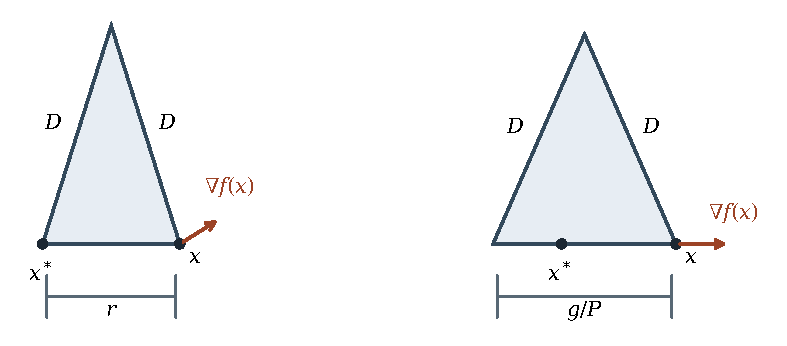
\includegraphics[width=0.9\linewidth]{figures/diameter_geometry.pdf}
\caption{Конструкции точности для допустимых точных наблюдений. Слева: активен зазор, $g\le P^2/m$. Справа: активна норма, $P^2/m<g\le PD$. Обе наклонные стороны имеют длину $D$.}
\label{jointdiam:geometry}
\end{figure}

\paragraph{Доказательство теоремы~\ref{jointdiam:main}.}
Из определения следует $0<\rho_-\le\rho_+$; непрерывность $V$
обеспечивает существование максимума. Для неоптимального источника
обозначим $r=\|x-x^*\|$, а через $p$ его конечную радиальную
производную. Сдвинутое RSI и условие минимума на области дают
$mr\le p\le P$; кроме того, $pr\le G(x)\le g$ и $r\le D$.
Следовательно,
\[
 pr\le\min\{g,P^2/m,PD\}=h,\qquad
 r\le R:=\min\{\sqrt{h/m},D\}.
\]
Положим $r_0=h/P\le R$. Радиальная огибающая $A(P,r)$ из
\eqref{joint:radial-identity} строго возрастает по $r$.
При $r\le r_0$ она ограничивает ошибку величиной
$A(P,r_0)=V(h,r_0^2)$. При $r\ge r_0$ верхние границы $h/r$
для конечной и $h/r-mr$ для начальной производной дают оценку
$V(h,r^2)$. Тем самым доказано \eqref{jointdiam:definition}.
Нулевой зазор или нулевая норма в силу сдвинутого RSI означают
нулевую ошибку. Нулевая оценка достигается в точке минимума
квадратичной функции на треугольнике диаметра $D$.

Для доказательства точности выберем максимизирующий радиус
$\rho$ и положим
\[
 r=\sqrt\rho,\quad p=h/r,\quad q=p-mr,\quad
 c=\sqrt{P^2-p^2},\quad a_D=\sqrt{D^2-r^2/4}.
\]
Скалярная конструкция из леммы~\ref{compact:radial}
даёт гладкие функции $u_j$ на окрестностях $[0,r]$ с условиями
\[
 \begin{gathered}
 u_j(0)=0,\quad u_j'(0)=q,\quad u_j'(r)=p,\quad
 u_j'(s)-q\ge ms,\\
 |u_j''(s)|\le H_0+H_1u_j(s),\qquad
 u_j(r)\longrightarrow V(h,\rho).
 \end{gathered}
\]
Определим
\[
 Q=\operatorname{conv}\{(0,0),(r,0),(r/2,a_D)\},\qquad
 f_j(s,y)=u_j(s)+cy+my^2/2.
\]
Две боковые стороны имеют длину $D$, а основание имеет длину
$r\le D$. Поэтому диаметр $Q$ равен ровно $D$, и внутренность
непуста. В его точках $0\le s\le r$ и $y\ge0$.
Единственная точка минимума есть $(0,0)$; всюду на $Q$
\[
 \langle\nabla f_j(s,y)-\nabla f_j(0,0),(s,y)\rangle
       =(u_j'(s)-q)s+my^2\ge m(s^2+y^2),
\]
\[
 \|\nabla^2f_j(s,y)\|
       =\max\{|u_j''(s)|,m\}
       \le H_0+H_1u_j(s)\le H_0+H_1f_j(s,y).
\]
В точке $(r,0)$ градиент равен $(p,c)$ и имеет норму $P$.
Его скалярное произведение с точками области минимально в
$(0,0)$, так что полный зазор равен $pr=h\le g$.
Ошибка источника стремится к $\mathcal J_D(g,P)$.
Это доказывает точность для верхних границ, в том числе при
точно заданном диаметре.

Для точных положительных наблюдений условие $g\le PD$
необходимо, поскольку
$G(x)\le\|\nabla f(x)\|\operatorname{diam}Q$.
Если также $g\le P^2/m$, то $h=g$, и предыдущая конструкция
уже задаёт оба наблюдения точно. Если $P^2/m<g\le PD$, положим
\[
 r=P/m,\qquad a=g/P-r,\qquad \ell=r+a=g/P\le D.
\]
Возьмём гладкие скалярные профили на $[0,r]$ с нулевой начальной
производной и конечной производной $P$, приближающие $\mathcal E(P)$.
Сглаживание затрагивает только внутреннее переключение,
поэтому около нуля они совпадают с
\[
 u_+(s)=
 \begin{cases}
 (H_0/H_1)\{\cosh(\sqrt{H_1}s)-1\},&H_1>0,\\
 H_0s^2/2,&H_1=0.
 \end{cases}
\]
Продолжим их на $[-a,0]$ этой чётной функцией. На добавленном
отрезке $|u_+''|=H_0+H_1u_+$ и $u_+'(s)s\ge ms^2$.
Обозначим продолжение через $u_j$. На треугольнике
\[
 Q=\operatorname{conv}\left\{(-a,0),(r,0),
       \left((r-a)/2,\sqrt{D^2-\ell^2/4}\right)\right\}
\]
положим $f_j(s,y)=u_j(s)+my^2/2$.
Снова $\operatorname{diam}Q=D$, точка минимума есть $(0,0)$,
а сдвинутое RSI и ограничение Гессиана выполнены на всём $Q$.
Градиент источника равен $(P,0)$; линейный оракул выбирает
$(-a,0)$ и даёт зазор $P\ell=g$. Ошибка стремится к
$\mathcal E(P)=\mathcal J_D(g,P)$.
Все функции гладкие на окрестностях своих треугольников.

Формула \eqref{jointdiam:constant} получается максимизацией
аффинной по радиусу функции $h+\beta\rho$.
Формула \eqref{jointdiam:ordinary} следует из
следствия~\ref{gapregime:radius-monotone} при $\rho_-$.
Для следствия~\ref{jointdiam:norm} граница зазора $PD$
следует из ограничений на норму и диаметр.
В $\mathcal J_D(PD,P)$ отрезок радиусов состоит из одной
точки $r_D^2$, а начальная производная равна
$P-mr_D=\max\{P-mD,0\}=q$.
Радиальное тождество и предложение~\ref{joint:fixed-slope}
дают \eqref{jointdiam:norm-formula}; формула радиальной
огибающей при постоянной кривизне даёт
\eqref{jointdiam:norm-constant}.

\paragraph{Полный зазор при известном диаметре.}
Для $D>0$ определим
\begin{equation}\label{compact:gap-diameter}
 \mathcal B_D(g)=
 \max_{0\le\rho\le\min\{g/m,D^2\}}V(g,\rho),\qquad
 \mathcal B_D(0)=0.
\end{equation}
При $\operatorname{diam}Q\le D$ имеем
$\delta(x)\le\mathcal B_D(G(x))\le\mathcal B(G(x))$.
Это точный супремум при фиксированном полном зазоре и границе
диаметра. Функция $\mathcal B_D$ непрерывна и удовлетворяет
\eqref{boundarygap:growth}.

Действительно, радиальная верхняя оценка использует $r\le D$,
а гладкие примеры на $[0,r]$ из леммы~\ref{compact:radial}
приближают все значения с $r\le D$.
Предел $\rho\downarrow0$ обеспечивают те же линейно-квадратичные
примеры, что в доказательстве теоремы~\ref{boundarygap:main}.
Замена $\rho=z\min\{g/m,D^2\}$, $z\in[0,1]$, доказывает
непрерывность; добавление линейного слагаемого доказывает рост,
не меняя длину отрезка.

При $H_1=0$
\[
 \mathcal B_D(g)=g+\max\{0,\beta\}\min\{g/m,D^2\}.
\]
При $H_1>0$, $g>0$ имеем точный критерий
\[
 \mathcal B_D(g)=g\quad\Longleftrightarrow\quad\mathcal S(g)\le0.
\]
При неположительном знаке достаточно
$g\le\mathcal B_D(g)\le\mathcal B(g)=g$.
При положительном знаке первая вариация
\eqref{gapregime:variation} превышает $g$ при сколь угодно
малых положительных радиусах, удовлетворяющих также $\rho\le D^2$.
Для скалярного вычисления применяется предложение~\ref{boundarygap:budget}
на укороченном отрезке с $\ell=g$.

\section{Адаптивная остановка и полный учёт запросов}
\label{nloracle:section}
Сертификаты выше совместимы с обычным квадратичным поиском шага.
Докажем общую оценку работы для калибровки $\Phi$.
Значения функции считаются точными.
Пусть $D\ge\operatorname{diam}Q>0$ и
\begin{equation}\label{nloracle:model}
 \lambda_{\max}(\nabla^2f(x))\le K(\delta(x)),\qquad
 \delta(x)\le\Phi(G(x)).
\end{equation}
Функция $K:[0,\infty)\to[0,\infty)$ конечна, непрерывна и не убывает,
а $\Phi:[0,\infty)\to[0,\infty)$ непрерывна, строго возрастает,
не ограничена сверху и удовлетворяет $\Phi(0)=0$.
Точной огибающей зазора соответствуют $\Phi=\mathcal B$ и
$K(u)=H_0+H_1u$. Условия \eqref{nloracle:model} допускают
и другие классы функций.
При известной границе диаметра можно также взять $\Phi=\mathcal B_D$.

При запрошенной точности направлений $\eta>0$ оракул возвращает
$h\ge0$ и $d=s-x$, $s\in Q$, для которых
\begin{equation}\label{nloracle:query}
 G(x)\le B=h+\eta,\qquad
 -\langle\nabla f(x),d\rangle\ge h-\eta.
\end{equation}
Сертификат в текущей точке должен удовлетворять
$\delta(x)\le C\le\Phi(B)$. Можно взять $C=\Phi(B)$
или более точную совместную границу.
Обновим $\ell\leftarrow\max\{\ell,f(x)-C\}$ и положим $U=f(x)-\ell$.
Первый запрос создаёт начальную нижнюю границу.

\paragraph{Правило.}
Выберем $\eta_0,M>0$, $0<\theta<1$ и будем переносить $\eta$
между точками. После каждого запроса сначала остановимся, если
$U\le\varepsilon$, где $\varepsilon>0$.
Иначе проверим $\eta\le\theta h$. Если условие не выполнено,
уменьшим $\eta$ вдвое и повторим запрос в той же точке,
используя сохранённое значение функции.
После успешной проверки положим $a=h-\eta$,
начнём с $L=L_{k-1}/2$, $L_{-1}=M$, и будем удваивать $L$, пока
\begin{equation}\label{eq:btstep}
 \alpha=\min\{1,a/(L\|d\|^2)\},\qquad
 f(x+\alpha d)\le f(x)-\alpha a+\tfrac12L\alpha^2\|d\|^2.
\end{equation}
Примем точку $x+\alpha d$, сохраним её значение и принятое $L_k$.
Сам поиск шага стандартен~\cite{pedregosa}; сертификаты определяют,
когда полученная точка достаточно точна.

\begin{theorem}[Остановка с переносом точности]\label{nloracle:main}
Каждый цикл уточнения и поиска шага конечен. Правило останавливается
с $\delta(x_N)\le U_N\le\varepsilon$.
Пусть $N$ есть число принятых обновлений, а $R$ есть число делений
точности пополам, включая начальную и последнюю проверки.
При $\kappa=(1-\theta)/(1+\theta)$
\begin{equation}\label{nloracle:refinement}
 R\le\left\lceil\log_2\max\left\{1,
 \frac{(1+\theta)\eta_0}{\theta\Phi^{-1}(\varepsilon)}\right\}\right\rceil,
 \qquad T=N+1+R.
\end{equation}
Запросов в текущих точках ровно $T$.
Каждый векторный запрос с полным LMO требует одного вызова LMO;
каждый запрос оценок атомов ниже требует одного полного прохода по ним.

Если нужно хотя бы одно обновление, пусть $U_0>\varepsilon$ есть
сертификат после начальной проверки точности. Положим
\[
 \begin{gathered}
 J=\lceil\log_2(U_0/\varepsilon)\rceil,\quad b_j=U_0/2^j,\quad
 s_j=\kappa\Phi^{-1}(b_j/2),\\
 C_j=\max\{2K(b_j),s_j/D^2\},\quad
 P_K=\left\lceil\log_2\frac{\max\{M,C_0\}}{C_{J-1}}\right\rceil,
 \qquad 0\le j<J.
 \end{gathered}
\]
Тогда
\begin{equation}\label{nloracle:work}
 N\le T_\varepsilon:=P_K+
 \left\lceil\sum_{j=0}^{J-1}
 \max\left\{\frac{2b_j}{s_j},\frac{4D^2K(b_j)b_j}{s_j^2}\right\}\right\rceil.
\end{equation}
При фактическом $N\ge1$ число вычислений функции, включая
начальное значение и отклонённые пробы, удовлетворяет
\begin{equation}\label{nloracle:functions}
 N_f\le1+2N+
 \left\lceil\log_2\max\{1,2K(U_0)/M\}\right\rceil.
\end{equation}
При $N=0$ требуется одно значение функции и $1+R$ запросов.
Фазовые величины в этом случае не нужны.
\end{theorem}

\begin{proof}
Каждая сохранённая нижняя граница верна, поэтому
$0\le\delta\le U\le C\le\Phi(B)$.
Если остановка ещё не выполнена, а проверка точности не прошла, то
\[
 \Phi^{-1}(\varepsilon)<\Phi^{-1}(U)\le B
   <(1+\theta)\eta/\theta.
\]
Точность уменьшается вдвое и не сбрасывается. Отсюда следуют
граница для $R$ и конечность уточнений.
В каждой посещённой точке один запрос завершает проверку,
а каждому делению точности соответствует один неудачный запрос.
Значит, $T=N+1+R$.
После успешной проверки перед обновлением
\begin{equation}\label{compact:certified-slope}
 a=h-\eta\ge\kappa(h+\eta)\ge\kappa\Phi^{-1}(U)>0.
\end{equation}

Для поиска шага положим $w(t)=f(x+td)-f(x)$,
$K_x=K(\delta(x))$.
Пока $w\le0$, имеем $w''\le K_x\|d\|^2$ и $w'(0)\le-a<0$.
Первый возврат к нулю до $2a/(K_x\|d\|^2)$ противоречил бы
$w(t)\le-at+K_x\|d\|^2t^2/2<0$.
Поэтому любое $L\ge K_x$ проходит проверку с предложенным шагом.
При $K_x=0$ достаточно линейного сравнения.
Каждая принятая проба удовлетворяет
\begin{equation}\label{eq:acceptedprogress}
 f_k-f_{k+1}\ge\alpha_k a_k/2,\qquad
 L_k\le\max\{L_{k-1}/2,2K(\delta_k)\}.
\end{equation}
Значение функции убывает, а нижняя граница не убывает.
Значит, $U$ не возрастает, в том числе при уточнениях в одной точке.

Отнесём обновление к фазе $b_j/2<U_k\le b_j$.
Положительные границы $C_j$ не возрастают.
Если $L_k>C_j$, принятая проба была первой: иначе предыдущее
отклонённое значение было бы не меньше $C_j/2\ge K(\delta_k)$.
Такое обновление уменьшает унаследованную кривизну вдвое.
Перед обновлением фазы $j$ рассмотрим потенциал
\[
 V_k=\max\{0,\log_2(L_{k-1}/C_j)\}.
\]
Обновление выше границы уменьшает его на единицу;
обновление не выше границы оставляет нулевое значение до смены фазы.
Переход из $j$ в $j'$ увеличивает потенциал не более чем на
$\log_2(C_j/C_{j'})$. Эти приращения телескопируются,
поэтому обновлений выше своих границ не больше $P_K$.

На остальных обновлениях \eqref{compact:certified-slope} и
$\|d\|\le D$ дают убывание функции не меньше
\[
 p_j=\min\{s_j/2,s_j^2/(2C_jD^2)\}=s_j^2/(2C_jD^2).
\]
Суммарное убывание от точек фазы $j$ не больше действительной
ошибки при входе в фазу, а она не больше $b_j$.
Таких обновлений не больше $b_j/p_j$.
Суммирование даёт \eqref{nloracle:work}.
Та же конечная граница верна для любого незавершённого префикса,
что исключает бесконечную работу без остановки.

Если на обновлении $k$ отклонено $q_k$ проб, то
$L_k=2^{q_k-1}L_{k-1}$. Следовательно,
\[
 \sum_{k<N}(q_k+1)=2N+\log_2(L_{N-1}/M),\qquad
 L_{N-1}\le\max\{M/2^N,2K(U_0)\}.
\]
Добавим начальное вычисление функции и получим
\eqref{nloracle:functions}.
\end{proof}

\paragraph{Шаги от активных атомов.}\label{alg:afw}
Для $Q=\operatorname{conv}\mathcal A$ с конечным набором атомов
поддерживаем точные положительные веса активного множества $S$.
В AFW полный LMO возвращает минимизирующий атом из $\mathcal A$,
в том числе при неоднозначном минимуме.
Для остановки и проверки точности FW используем $B=h_{\rm FW}+\eta$.
Только после успешной проверки просматриваем активное множество
и сравниваем его приближённый зазор away с зазором FW.
Выбираем больший; при равенстве или одном активном атоме используем FW.
Из выбранного зазора вычитаем $\eta$.
Гарантия ошибки должна одновременно покрывать оба направления,
как в следующем разделе.
Для направления $x-v$ предельный шаг равен $\lambda_v/(1-\lambda_v)$;
заменим им ограничение $1$ в \eqref{eq:btstep}~\cite{lacostejaggi}.
Шаг, достигший этого предела, удаляет атом.
Каждый другой шаг имеет ту же границу продвижения, что и FW.
Потенциальный аргумент считает все обновления выше границ $C_j$,
а аргумент через убывание считает остальные хорошие обновления.
Поэтому хороших обновлений не больше $T_\varepsilon$.
FW добавляет не больше одного атома, а удаление убирает один, откуда
\begin{equation}\label{eq:dropcount}
 N\le2T_\varepsilon+|S_0|-1.
\end{equation}
Границы запросов и значений функции используют фактическое полное $N$.
Дополнительно AFW выполняет $N$ просмотров активного множества.

\begin{corollary}[Скалярное вычисление с доказанной точностью]
\label{nloracle:energy}
Пусть $\delta\le\Phi_0(G)$, а скалярная процедура возвращает
$\Phi_0(B)\le\widehat\Phi_0(B)\le\vartheta\Phi_0(B)$
с известным $\vartheta\ge1$.
Возьмём $C=\widehat\Phi_0(B)$ либо минимум этого значения и
другой корректной верхней границы ошибки в текущей точке.
Теорема применима с $\Phi=\vartheta\Phi_0$.
В частности, можно взять $\Phi_0=\mathcal B$ или $\Phi_0=\mathcal B_D$, а при
$\nabla f(x^*)=0$ также $\Phi_0=W$.
Обратная функция нужна в анализе, а не в алгоритме.
\end{corollary}
\begin{proof}
Корректность даёт $\delta\le C$, а построение даёт
$U\le C\le\vartheta\Phi_0(B)$.
Это именно калибровочные неравенства, использованные в доказательстве.
Нужные свойства $\mathcal B$ и $W$ уже доказаны.
\end{proof}

Нормовая граница $P^+$ позволяет выбрать точный
$C=\mathcal J_D(B,P^+)$.
При вычисленном верхнем включении используем
$C=\widehat{\mathcal J}_D(B,P^+)\le\vartheta\mathcal J_D(B,P^+)
\le\vartheta\mathcal B_D(B)$ и эффективную калибровку
$\Phi=\vartheta\mathcal B_D$.
Последнее неравенство следует из точности $\mathcal J_D$
в классе с верхними границами наблюдений.
Оба варианта можно объединить с другими корректными границами
в текущей точке, взяв их минимум.
Вычисление нормы и скалярного сертификата оплачивается отдельно.
Если на запросе $j$ процедура использует $n(B_j)$ сравнений,
учитывается $\sum_{j=1}^{N+1+R}n(B_j)$, включая неудачные уточнения
и последнюю проверку. Счёт сравнений не ограничивает стоимость
интервальной или битовой арифметики.
Для невозрастающей границы стоимости запроса $C_{\rm query}(\eta)$
общая стоимость не больше
\[
 (N+1)C_{\rm query}(\eta_R)+\sum_{r=0}^{R-1}C_{\rm query}(\eta_0 2^{-r}).
\]

\paragraph{Линейная граница зазора и последние фазы.}
Из известной оценки $G\ge\gamma\delta$, $\gamma>0$, получаем
$\Phi(g)=g/\gamma$.
При $K(u)=H_0+H_1u$ и $\bar\gamma=\kappa\gamma$
\eqref{nloracle:work} даёт
\[
 N\le P_K+\left\lceil
 \frac{4J}{\bar\gamma}+
 \frac{32D^2H_0}{\bar\gamma^2\varepsilon}+
 \frac{16D^2H_1J}{\bar\gamma^2}\right\rceil.
\]
Действительно, $s_j=\bar\gamma b_j/2$ и
$\sum_{j<J}b_j^{-1}<2/\varepsilon$.
Квазар-выпуклость с центром $x^*$
даёт эту оценку через
$\langle\nabla f(x),x-x^*\rangle\ge\gamma\delta(x)$.
Она не требует выпуклости между произвольными парами точек.
Для точной калибровки при сдвинутом RSI фазы с $b_j/2\le g_c$
имеют $\mathcal B^{-1}(b_j/2)=b_j/2$, если положительный порог
$g_c$ существует. Их граница продвижения имеет ту же форму с $\gamma=1$.
Для $\Phi=\vartheta\mathcal B$ соответствующее условие имеет вид
$b_j/(2\vartheta)\le g_c$, а $s_j=\kappa b_j/(2\vartheta)$.
Те же формулы последних фаз верны для $\mathcal B_D$,
поскольку её диапазон обычного зазора совпадает с диапазоном $\mathcal B$.

\section{Направленные ошибки и наблюдения с конечной дисперсией}
\label{diroracle:section}
Дадим две реализации \eqref{nloracle:query} и один способ получения
наблюдений. Медиана средних является стандартной конструкцией~\cite{dirlugosi};
робастные стохастические варианты FW изучаются
в~\cite{dirtang,dirsfyraki}. Здесь она обеспечивает сертификат
глобальной ошибки при точных значениях функции.

\begin{proposition}[Векторные наблюдения и оценки атомов]
\label{diroracle:width-transfer}\label{diroracle:scores}
Определим полунорму допустимых направлений
\[
 \omega_Q(v)=\max_{u,w\in Q}\langle v,u-w\rangle\le D\|v\|.
\]
Если векторный запрос удовлетворяет
$\omega_Q(\widehat g-\nabla f(x))\le\eta$, выберем
$s\in\arg\min_{v\in Q}\langle\widehat g,v\rangle$ и
$h=\langle\widehat g,x-s\rangle$.
Тогда выполнено \eqref{nloracle:query}; гарантия верна и для
выбранного направления away с его приближённым зазором.

Пусть вместо этого $Q=\operatorname{conv}\{v_0,\ldots,v_{n_A-1}\}$,
$n_A\ge2$, а $x=\sum_i\lambda_i v_i$ задана точными неотрицательными
весами с суммой один. Положим
$t_i=\langle\nabla f(x),v_i-v_0\rangle$.
Предположим, что $q_0=t_0=0$ и
\begin{equation}\label{diroracle:score-error}
 \max_i(q_i-t_i)-\min_i(q_i-t_i)\le\eta.
\end{equation}
Возьмём $q_x=\sum_i\lambda_iq_i$, выберем
$i_s\in\arg\min_i q_i$ и положим $h=q_x-q_{i_s}$.
Это также даёт \eqref{nloracle:query} и гарантию для направления away.
Оценки $q_i$ не обязаны быть значениями одного линейного функционала.
Каждый запрос требует полного просмотра $n_A$ оценок.
\end{proposition}
\begin{proof}
Полунорма ограничивает абсолютную ошибку на разности любых
допустимых точек величиной $\eta$.
Максимизация даёт границу зазора; подстановка выбранного направления
даёт границу наклона.
Для оценок атомов положим $e_i=q_i-t_i$,
$e_x=\sum_i\lambda_i e_i$.
Число $e_x$ лежит между наименьшим и наибольшим $e_i$, поэтому
\[
 \langle\nabla f(x),x-v_i\rangle=q_x-q_i-e_x+e_i\le h+\eta.
\]
Выбранный наклон FW не меньше $h-\eta$, а наклон away
не меньше $q_i-q_x-\eta$.
Кроме того, $h\ge0$, поскольку $q_x$ есть выпуклая комбинация оценок.
\end{proof}

При евклидовой границе ошибки $\eta_{\rm norm}$ можно взять
$\eta=D\eta_{\rm norm}$ и $P^+=\|\widehat g\|+\eta_{\rm norm}$.
Последняя граница позволяет использовать совместный сертификат.
Из одних направленных ошибок или ошибок оценок атомов граница
нормы не следует.
Для шара $\ell_1$ радиуса $R$ имеем $\omega_Q(v)=2R\|v\|_\infty$;
для симплекса она равна $\max_i v_i-\min_i v_i$.
Перебор оценок не считается одним вызовом LMO на неявно заданном многограннике.

Пусть одно новое наблюдение в запрошенной точке даёт $n_A-1$
скалярных значений $Y_i$.
Условно на всём прошлом $\mathcal F$ наблюдения внутри запроса
независимы и одинаково распределены, с известной общей границей
\begin{equation}\label{diroracle:moment}
 \mathbb E[Y_i\mid\mathcal F]=t_i(x),\qquad
 \mathbb E[(Y_i-t_i(x))^2\mid\mathcal F]\le\sigma_A^2<\infty.
\end{equation}
Координаты одного наблюдения могут зависеть друг от друга.
Пронумеруем все запросы, включая уточнения, числами $j\ge1$.
На уровне точности $r$ положим $\eta_r=\eta_0 2^{-r}$ и
\begin{equation}\label{diroracle:batch}
 b_r=\max\{1,\lceil16\sigma_A^2/\eta_r^2\rceil\},\qquad
 k_j=2\left\lceil4\log\frac{(n_A-1)j(j+1)}\zeta\right\rceil+1,
 \quad 0<\zeta<1.
\end{equation}
Возьмём $b_rk_j$ наблюдений.
Для каждой координаты вычислим медиану средних по $k_j$
непересекающимся блокам размера $b_r$ и положим $q_0=0$.

\begin{theorem}[Единое событие доверия для всех запросов]
\label{diroracle:sampling}
С вероятностью не меньше $1-\zeta$ каждый запрос алгоритма
удовлетворяет \eqref{diroracle:score-error}.
На этом событии верны все оценки теоремы~\ref{nloracle:main},
включая $\delta(x_N)\le U_N\le\varepsilon$ в случайный момент остановки.
При фактическом $T=N+1+R$ число исходных наблюдений удовлетворяет
\begin{align}\label{diroracle:samples}
 S&\le k_T\left[(N+1)b_R+\sum_{r=0}^{R-1}b_r\right]\\
  &\le k_T\left[T+16\sigma_A^2\eta_R^{-2}
       \left(N+1+\frac{1-4^{-R}}3\right)\right].\nonumber
\end{align}
Каждое наблюдение возвращает все $n_A-1$ координат, то есть
получено $(n_A-1)S$ скалярных направленных значений.
Медианы, просмотры и точные вычисления функции учитываются отдельно.
\end{theorem}
\begin{proof}
Условное неравенство Чебышёва ограничивает вероятность ошибки
одного среднего больше $\eta_r/2$ величиной $1/4$.
При $\sigma_A=0$ эта вероятность нулевая.
Независимость блоков и неравенство Хёффдинга дают вероятность
ошибки нечётной медианы не больше $e^{-k_j/8}$.
Суммирование по координатам даёт условную вероятность неудачи
не больше $\zeta/[j(j+1)]$.
Если все координатные ошибки не превосходят $\eta_r/2$,
их размах не превосходит $\eta_r$, что даёт
\eqref{diroracle:score-error}.
Применим эту оценку на событии, что запрос $j$ сделан,
возьмём ожидание и просуммируем по всем $j\ge1$.
Так как сумма $1/[j(j+1)]$ равна единице, все запросы верны
одновременно с вероятностью не меньше $1-\zeta$.
Детерминированное доказательство для каждого префикса обеспечивает
конечную остановку без заранее заданного числа запросов.

На каждом уровне $0,\ldots,R-1$ имеется один неудачный запрос,
а $N+1$ завершающих запросов имеют уровни не больше $R$.
Монотонность $k_j$ даёт первую оценку числа наблюдений.
Для второй используем $b_r\le1+16\sigma_A^2\eta_r^{-2}$ и
$\sum_{r<R}\eta_r^{-2}=\eta_R^{-2}(1-4^{-R})/3$.
\end{proof}

Конечная дисперсия направленных наблюдений возможна без конечного
момента векторного наблюдения.
На симплексе общая компонента Коши $W\mathbf1$ сокращается
в каждой разности $\langle Z,e_i-e_0\rangle$.
Сами разности всё равно должны удовлетворять условной границе
дисперсии \eqref{diroracle:moment}.
Конструкция требует конечного явного набора атомов, новых выборок,
известной границы дисперсии и точных значений функции.

\section{Приложение к реализуемой сигмоидной регрессии}
\label{reg:sigmoid}
Квазар-выпуклость для реализуемых обобщённых
линейных моделей известна \cite[лемма 3]{regglm}; связь через отношение
производных также используется в \cite[лемма 5]{regfoster}.
Сигмоидные наименьшие квадраты на $\ell_1$-шаре уже применяются
для проверки методов условного градиента \cite[раздел 5.1.4]{khademi}.
Ниже даны явные константы для полученных сертификатов.

Пусть строки $A\in\mathbb R^{n\times d}$ равны $a_i^\top$,
$Q=\{x:\|x\|_1\le R\}$, $R>0$, и $x^*\in Q$.
Для $\sigma(z)=(1+e^{-z})^{-1}$ и ответов
$y_i=\sigma(a_i^\top x^*)$ положим
\begin{equation}\label{reg:sigmoidloss}
 f(x)=\frac1{2n}\sum_{i=1}^n[\sigma(a_i^\top x)-y_i]^2.
\end{equation}
Тогда $f^*=0$ и $\nabla f(x^*)=0$. Обозначим
\[
 \begin{gathered}
 Z=R\max_i\|a_i\|_\infty,\qquad
 m_\sigma=(2+2\cosh Z)^{-1},\quad
 M_\sigma=1/4,\quad C_\sigma=1/(6\sqrt3),\\
 S=A^\top A/n,\quad \lambda=\lambda_{\min}(S),\quad
 \Lambda=\lambda_{\max}(S),\quad K_A=\max_i\|a_i\|^2.
 \end{gathered}
\]
Все допустимые скалярные аргументы лежат в $[-Z,Z]$, где
$m_\sigma\le\sigma'\le M_\sigma$; на всей прямой
$|\sigma''|\le C_\sigma$.

\begin{proposition}[Константы регулярности и кривизны]
\label{reg:sigmoidbounds}
При $\lambda>0$ функция удовлетворяет сдвинутому RSI с
$m=m_\sigma^2\lambda$. Для каждого $t>0$ граница нормы гессиана
выполнена с
\begin{equation}\label{reg:sighess}
 H_0=\Lambda\left(M_\sigma^2+\frac{C_\sigma^2}{2t}\right),
 \qquad H_1=K_A t.
\end{equation}
Кроме того,
\begin{equation}\label{reg:quasar}
 \langle\nabla f(x),x-x^*\rangle\ge\gamma f(x),\qquad
 \gamma=\min\{1,2m_\sigma/M_\sigma\}>0,
\end{equation}
и на всей допустимой области
\begin{equation}\label{reg:sigglobal}
 \|\nabla^2f(x)\|\le L_Q
 :=\Lambda\bigl(M_\sigma^2+C_\sigma\tanh(Z/2)\bigr).
\end{equation}
Для последних двух выводов полный столбцовый ранг не требуется.
\end{proposition}
\begin{proof}
Положим $d=x-x^*$, $z_i=a_i^\top x$ и
$r_i=\sigma(z_i)-\sigma(a_i^\top x^*)$.
По теореме о среднем $r_i=\bar s_i a_i^\top d$, где
$\bar s_i\in[m_\sigma,M_\sigma]$. Поэтому
\[
 \langle\nabla f(x),d\rangle
 =\frac1n\sum_i\bar s_i\sigma'(z_i)(a_i^\top d)^2
 \ge m_\sigma^2d^\top Sd\ge m\|d\|^2.
\]
Та же сумма равна
$n^{-1}\sum_i\sigma'(z_i)r_i^2/\bar s_i
 \ge 2m_\sigma f(x)/M_\sigma$, что доказывает \eqref{reg:quasar}.
Гессиан имеет вид
\[
 \nabla^2f(x)=\frac1n\sum_i
 [\sigma'(z_i)^2+r_i\sigma''(z_i)]a_i a_i^\top.
\]
Для единичного $v$ неравенство Коши-Буняковского и оценка
$(a_i^\top v)^4\le K_A(a_i^\top v)^2$ ограничивают модуль
квадратичной формы величиной
\[
 M_\sigma^2\Lambda+C_\sigma\sqrt{2K_A\Lambda f(x)}
 \le\Lambda\left(M_\sigma^2+\frac{C_\sigma^2}{2t}\right)+K_Atf(x).
\]
Получена \eqref{reg:sighess}. Подстановка
$|r_i|\le\tanh(Z/2)$ даёт \eqref{reg:sigglobal}.
\end{proof}

Приложение включает невыпуклые функции. Возьмём $n=d=1$,
$Q=[-2,2]$, $a_1=1$ и $x^*=-2$. При
$q=\tanh1>1/2$ и $p=\sigma'(2)=(1-q^2)/4$ имеем
\[
 f''(2)=p^2-pq^2=\frac p4(1-5q^2)<0.
\]
По непрерывности кривизна отрицательна и в близких внутренних точках.

Константы требуют точной реализуемости. Для произвольных зашумлённых
ответов эти RSI и связь градиента с ошибкой без остаточного члена
не следуют. При большом $Z$ величина $m_\sigma$ может быть очень
малой, и оценки становятся консервативными. Аффинная граница
кривизны и $L_Q$ обе корректны; ни одна из них не всегда лучше.
Параметр $t$ задаёт границу, а не подбор шага.

Диаметр $\ell_1$-шара равен $D=2R$. Поэтому полный столбцовый ранг
позволяет применять все оценки по норме, зазору и их сочетанию,
включая $\mathcal J_D$; одной \eqref{reg:quasar} достаточно для
остановки с линейной связью ошибки и зазора. Если алгоритму известно,
что ответы реализуемы в допустимой точке, ему уже известно $f^*=0$,
и само значение $f(x)$ равно ошибке. Если при сравнении эта
нижняя граница скрыта, это нужно явно указать. Для произвольной
невыпуклой функции ограниченная задача не объявляется эквивалентной
задаче с фиксированным $\ell_1$-штрафом.

\section{Вычисление сертификатов и контрольные результаты}
\label{compact:evidence}
Доказательства устанавливают точные границы; вычисления ниже
проверяют формулы и реализацию. Глобальные максимумы не выводятся
из выборки радиусов. Код использует точные рациональные входы,
интервальную арифметику с округлением наружу, явные ограничения
ресурсов и отдельный статус отказа, если результат не удалось
сертифицировать.

\begin{table}[htbp]
\centering
\caption{Фиксированные сравнения сертификатов. Первая и третья строки
точны. Во второй сокращённо записан гарантированный интервал.}
\label{compact:certificate-table}
\begin{tabular}{lccc}
\toprule
$(m,H_0,H_1;g,P)$ & Отдельные оценки & $\mathcal J(g,P)$ & $\mathcal J_D(g,P)$\\
\midrule
$(1,1,0;1/2,1)$ & $1/2$ & $3/8$ & не используется\\
$(1,1,1;1,2)$ & $1$ & $0.903217\ldots$ & не используется\\
$(1,4,0;1,2)$ & $23/16$ & $23/16$ & $463/400$ при $D=3/5$\\
\bottomrule
\end{tabular}
\end{table}
Под отдельными оценками понимается
$\min\{\mathcal B(g),\mathcal E(P)\}$.
Для второй строки фиксированный скалярный расчёт дал
\[
 \begin{aligned}
 0.90321723720789&<\mathcal J(1,2)<0.90321723720790,\\
 2.56989673908727&<\mathcal E(2)<2.56989673908729.
 \end{aligned}
\]
Оценка по зазору равна единице. Алгебраическая верхняя граница
$2-7\sqrt{14}/24=0.908683\ldots$ также её улучшает.
Монотонность по радиусу доказывает, что выбранный конец отрезка
даёт совместный максимум. Расчёт использует 100 десятичных знаков
и 96 шагов бисекции переключения для каждого фиксированного
радиуса; запись содержит независимые включения времени прохождения.
В примере с диаметром выполнено $g<PD$, поэтому улучшение сохраняется
и при точном задании обоих наблюдений.

Сохранённый протокол API v16 содержит 16 заданных вызовов,
12 сертификатов и четыре ожидаемых отказа, а контрольный скрипт
выполнил 238 проверок. Более ранний протокол v15 с 26 вызовами
и 503 проверками хранится отдельно. Это не числа экспериментов
оптимизации. Отдельный первый запуск расширения с диаметром
содержит десять заданных вызовов: семь сертификатов, три ожидаемых
отказа и 184 проверки контрольного скрипта. Выполнены 113 учитываемых
скалярных вычислений и 61 шаг бисекции. Файл проверок выпуска
содержит отдельные исходы и счётчики операций.
API отклоняет двоичные числа с плавающей точкой,
чтобы не принимать округлённые наблюдения за точные.
Отказ вычислителя не опровергает аналитическую границу.

Записи прежних оптимизационных исследований хранятся в отдельном
архиве. Например, фиксированный эмпирический монитор
сертифицировал пять из 16 сохранённых траекторий, а отдельное
исследование шести отобранных конечных точек дало три сертификата.
Правила отбора различались, поэтому результаты не объединяются.
Эти исследования относятся к прежним прикладным мониторам,
а не к проверке скорости $\mathcal J_D$. В данной редакции нет
новых траекторий оптимизации, решений ЛП или случайных выборок.
Проверки формул и статьи учитываются отдельно от затрат
оптимизационного алгоритма.

\section{Границы применимости и дальнейшие вопросы}
Точные оценки используют известные константы регулярности и кривизны.
Оценивание этих констант по конечной выборке производных не проверяет
условия на всей допустимой области. Для сигмоидного приложения
константы выведены из модели; другим приложениям нужно отдельное
обоснование.

Диаметр усиливает наилучшую оценку в классе меняющихся областей.
Фиксированный многогранник, известная активная грань или дополнительные
значения производных могут содержать больше информации, чем
$(g,P,D)$. Поиск точных сертификатов с такими данными остаётся
отдельной задачей. Возможная невогнутость радиального профиля также
оставляет вопрос о гарантированной максимизации, более экономной,
чем общая конечная сетка.

Теорема об остановке предполагает точные значения функции.
Её случайная реализация дополнительно требует новых направленных
наблюдений, конечного явно заданного множества атомов и известной
границы дисперсии. Для зашумлённых значений функции и неизвестных
дисперсий нужен дополнительный анализ. Счёт скалярных сравнений
не даёт битовую сложность или время интервальных вычислений.

\paragraph{Воспроизводимость.}
В выпуск входят исходники обеих статей, код сертификатов,
фик\-си\-ро\-ван\-ные скалярные протоколы и записи первых запусков.
Прежние расширенные доказательства и записи вычислений
сохранены в отдельном архиве.

\paragraph{Использование ИИ.}
Инструменты ИИ использовались для математических черновиков, кода,
перевода и редактуры. Зафиксированные проверки являются численными
или аналитическими разборами, а не формальной верификацией доказательств.

\begin{thebibliography}{99}
\bibitem{warmup}F.~Alimisis, R.~Islamov, and A.~Lucchi.
Why Do We Need Warm-up? A Theoretical Perspective.
\href{https://arxiv.org/abs/2510.03164v2}{arXiv:2510.03164v2}, 2026.

\bibitem{vyguzov}A.~A.~Vyguzov, F.~S.~Stonyakin, and A.~V.~Gasnikov.
Frank-Wolfe Algorithms for $(L_0,L_1)$-smooth functions.
\emph{Journal of Nonlinear and Variational Analysis}, 10(3):597-616, 2026.
\href{https://doi.org/10.23952/jnva.10.2026.3.05}{doi:10.23952/jnva.10.2026.3.05}.

\bibitem{regregularity}Y.~Zhou and Y.~Liang.
Characterization of Gradient Dominance and Regularity Conditions for Neural Networks.
\href{https://arxiv.org/abs/1710.06910v2}{arXiv:1710.06910v2}, 2017.

\bibitem{rsipep}C.~Guille-Escuret, A.~Ibrahim, B.~Goujaud,
and I.~Mitliagkas.
Gradient Descent Is Optimal Under Lower Restricted Secant Inequality
And Upper Error Bound.
\emph{Advances in Neural Information Processing Systems}, 35, 2022.
\href{https://proceedings.neurips.cc/paper_files/paper/2022/file/9daab3b451038ed1bc5d8e9b77996b99-Paper-Conference.pdf}{NeurIPS proceedings}.

\bibitem{pedregosa}F.~Pedregosa, G.~Negiar, A.~Askari, and M.~Jaggi.
Linearly Convergent Frank-Wolfe with Backtracking Line-Search.
\emph{AISTATS}, 2020. \href{https://arxiv.org/abs/1806.05123}{arXiv:1806.05123}.

\bibitem{lacostejaggi}S.~Lacoste-Julien and M.~Jaggi.
On the Global Linear Convergence of Frank-Wolfe Optimization Variants.
\emph{NeurIPS}, 2015.
\href{https://arxiv.org/abs/1511.05932}{arXiv:1511.05932}.

\bibitem{oraclehallak}N.~Hallak and K.~Y.~Levy.
A Study of First-Order Methods with a Deterministic Relative-Error Gradient Oracle.
\emph{Proceedings of the 41st International Conference on Machine Learning},
PMLR 235:17313-17332, 2024.
\url{https://proceedings.mlr.press/v235/hallak24a.html}.

\bibitem{oracledenisov}G. Denisov, F. Stonyakin, and M. Alkousa.
Adaptive Variants of Frank-Wolfe Method with Relative Inexact
Gradient Information.
\emph{Mathematical Optimization Theory and Operations Research},
LNCS 15681, pp. 3 to 16, 2025.
\url{https://doi.org/10.1007/978-3-031-97077-1_1}.

\bibitem{dirlugosi}G. Lugosi and S. Mendelson.
Mean estimation and regression under heavy-tailed distributions: a survey.
\emph{Foundations of Computational Mathematics}, 19:1145-1190, 2019.
\href{https://arxiv.org/abs/1906.04280}{arXiv:1906.04280}.

\bibitem{dirtang}T. Tang, K. Balasubramanian, and T. C. M. Lee.
High-probability bounds for robust stochastic Frank-Wolfe algorithm.
\emph{Proceedings of the Thirty-Eighth Conference on Uncertainty in
Artificial Intelligence}, PMLR 180:1917-1927, 2022.
\href{https://proceedings.mlr.press/v180/tang22a.html}{Publisher page}.

\bibitem{dirsfyraki}M.-E. Sfyraki and J.-K. Wang.
Lions and Muons: Optimization via stochastic Frank-Wolfe under
heavy-tailed noise.
\emph{Proceedings of the 43rd International Conference on Machine
Learning}, PMLR 306:109388-109428, 2026.
\href{https://proceedings.mlr.press/v306/sfyraki26a.html}{Publisher page}.

\bibitem{regglm}J.-K.~Wang and A.~Wibisono.
Continuized Acceleration for Quasar Convex Functions in Non-Convex Optimization.
\emph{ICLR}, 2023.
\href{https://arxiv.org/abs/2302.07851}{arXiv:2302.07851}.

\bibitem{regfoster}D.~J.~Foster, A.~Sekhari, and K.~Sridharan.
Uniform Convergence of Gradients for Non-Convex Learning and Optimization.
\emph{Advances in Neural Information Processing Systems}, 31, 2018.
\href{https://arxiv.org/abs/1810.11059v2}{arXiv:1810.11059v2}.

\bibitem{khademi}A.~Khademi and A.~Silveti-Falls.
Adaptive Conditional Gradient Descent.
\href{https://arxiv.org/abs/2510.11440v1}{arXiv:2510.11440v1}, 2025.
\end{thebibliography}

\end{document}
